\chapter{两角和与差的三角函数}
我们已经学习了任意角的三角函数及其性质、图象,这一章我们将要进一步学习两角和、差以及倍角、半角的三角
函数,并将学习三角式的和差化积、积化和差变形和简单的三角方程。
\section{两角和与差的三角函数}
\subsection{两角的和与差}
设$\alpha$、$\beta$为两个任意实数,它们
分别表示两个角的数量。那么实数$\alpha+\beta$就表示这两个角的和角的数量。两个角的和角可以做加法得到,即,以角$\alpha $的终边为始边,再旋转出一个角$\beta$(若$\beta>0$, 按逆时针方向旋转;若$\beta<0$, 按顺时针方向旋转),这时,以$\alpha $角的始边为始边,以$\beta$角的终边为终边的角,就是角$\alpha +\beta$. 两个角的差角可以由减法得出,角的减法是加法的逆运算,即$(\alpha -\beta)+\beta=\alpha$.

两个角的差角,也可以表示成和角的形式,如$\alpha -\beta=\alpha + (-\beta)$.

两个弧的和与差可按它们所对应的圆心角的和与差的法则来完成。

\begin{ex}
    试画图表示出以下的和角、差角:
    \[\alpha=30^{\circ},\quad \beta=45^{\circ}; \qquad \alpha=\frac{\pi}{3},\quad \beta=-\frac{3\pi}{4}   \]
\end{ex}

\subsection{两角和与差的余弦}
两角和与差的余弦函数,可以利用每个单角的三角函数来表示。

\begin{blk}{定理1}
    两个任意角$\alpha$, $\beta$的和(或差)的余弦,等于这两个角的余弦的乘积减去(或加上)这两个角的正弦的乘积。即
\begin{align}
    \cos (\alpha+\beta) &=\cos\alpha\cos\beta-\sin\alpha\sin\beta\\
\cos (\alpha-\beta) &=\cos\alpha\cos\beta+\sin\alpha\sin\beta
\end{align}
\end{blk}
 
\begin{proof}
我们先来证公式(1.2)。

设$\alpha,\beta$为任意两个给定的角(不论大小及正负),
把它们的始边都放在$x$轴正半轴,而终边与单位圆的交点分别为$P_1$, $P_2$(图1.1).

\begin{figure}[htp]
    \centering
    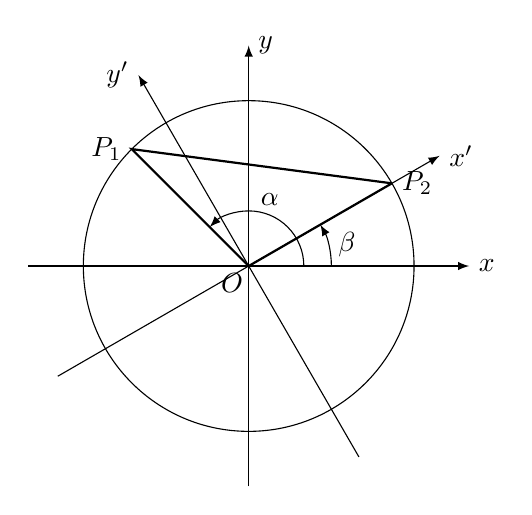
\begin{tikzpicture}[>=latex, scale=.7]
\draw[->] (-4,0)--(4,0)node[right]{$x$};
\draw[->] (0,-4)--(0,4)node[right]{$y$};
\draw (0,0) circle (3);
\draw [->] (210:4)--(30:4)node[right]{$x'$};
\draw [<-] (120:4)node[left]{$y'$}--(-60:4); 
\draw[thick](30:3)node[right]{$P_2$}--(135:3)node[left]{$P_1$}--(0,0)--(30:3);
\draw[->] (1.5,0) arc (0:30:1.5);
\draw [->] (1,0) arc (0:135:1);
\node at (67.5:1)[above]{$\alpha$};
\node at (15:1.5)[right]{$\beta$};
\node at (-.3,-.3){$O$};


    \end{tikzpicture}
    \caption{}
\end{figure}

把$Ox$轴旋转到$\beta$的终边位置而成$Ox'$轴,$Oy$轴旋转同样的角而成$Oy'$轴,
我们用两种方法计算弦长$P_1$, $P_2$。

在$x'Oy'$坐标系中,$P_1$, $P_2$的坐标是
\[P_1\; \left(\cos(\alpha-\beta),\, \sin(\alpha-\beta)\right),\qquad P_2\; (1,0) \]
利用两点间距离公式,得:
\begin{equation}
\begin{split}
|P_1P_2|^2 &=\left[\cos(\alpha-\beta)-1\right]^2+\left[\sin(\alpha-\beta)-0\right]^2\\
&=\cos^2(\alpha-\beta)-2\cos(\alpha-\beta)+1+\sin^2(\alpha-\beta)\\
&=2-2\cos (\alpha-\beta)
\end{split}
\end{equation}

在$xOy$坐标系中,$P_1$, $P_2$的坐标是
\[P_1\;(\cos\alpha,\, \sin\alpha),\qquad  P_2\; (\cos\beta,\, \sin\beta)\]
利用两点间距离公式,得:
\begin{equation}
    \begin{split}
    |P_1P_2|^2 &=(\cos\alpha-\cos\beta)^2+(\sin\alpha-\sin\beta)^2\\
    &=\cos^2\alpha-2\cos\alpha\cos\beta+\cos^2\beta +\sin^2\alpha-2\sin\alpha\sin\beta+\sin^2\beta\\
    &=2-2(\cos\alpha\cos\beta+\sin\alpha\sin\beta)
    \end{split}
    \end{equation}

    在两个坐标系下,弦长是不变的,比较(1.3)式和(1.4)式,即得
   \[ \cos (\alpha-\beta) =\cos\alpha\cos\beta+\sin\alpha\sin\beta\]
    这就是我们所要证明的。
\end{proof}

既然公式(1.2)对任意$\alpha$, $\beta$都成立,则以$-\beta$代替$\beta$, 也必成立
    \[ \cos [\alpha-(-\beta)] =\cos\alpha\cos(-\beta)+\sin\alpha\sin(-\beta)\]

再注意三角函数的奇偶性,就得到
\[ \cos(\alpha+\beta) =\cos\alpha\cos\beta-\sin\alpha\sin\beta\]
这就是我们所要证明的公式(1.1)。

\begin{example}
不查表,求$\cos15^{\circ}$, $\cos75^{\circ}$的值。
\end{example}

\begin{solution}
由于:$15^{\circ}=45^{\circ}-30^{\circ},\qquad 75^{\circ}=45^{\circ}+30^{\circ}$
\[\cos 45^{\circ}=\sin 45^{\circ}=\frac{\sqrt{2}}{2},\quad \cos 30^{\circ}=\frac{\sqrt{3}}{2},\quad \sin 30^{\circ}=\frac{1}{2} \]
所以:
\[\begin{split}
\cos15^{\circ}&=\cos(45^{\circ}-30^{\circ})=\cos 45^{\circ}\cos30^{\circ}+\sin 45^{\circ}\sin30^{\circ}\\
&=\frac{\sqrt{2}}{2}\cdot \frac{\sqrt{3}}{2}+\frac{\sqrt{2}}{2}\cdot \frac{1}{2}\\
&=\frac{\sqrt{6}+\sqrt{2}}{4}\approx 0.9659 
\end{split}\]
\[\begin{split}
\cos75^{\circ}&=\cos(45^{\circ}+30^{\circ})=\cos 45^{\circ}\cos30^{\circ}-\sin 45^{\circ}\sin30^{\circ}\\
&=\frac{\sqrt{2}}{2}\cdot \frac{\sqrt{3}}{2}-\frac{\sqrt{2}}{2}\cdot \frac{1}{2}\\
&=\frac{\sqrt{6}-\sqrt{2}}{4}\approx \frac{2.4495-1.4142}{4}\\
&\approx 0.2588 
\end{split}\]
\end{solution}

\begin{example}
    已知$\sin\alpha=\frac{2}{3}$, $\cos\beta=-\frac{3}{4}$, 并且$\alpha$是第二象限的角,$\beta$是第三象限的角,求$\cos(\alpha-\beta)$的值(准确到0.01)。
\end{example}

\begin{solution}
因为$\alpha$是第二象限的角,所以
\[\cos\alpha=-\sqrt{1-\sin^2\alpha}=-\sqrt{1-\left(\frac{2}{3}\right)^2}=-\frac{\sqrt{5}}{3}\]
因为$\beta$是第三象限的角,所以
\[\sin\beta=-\sqrt{1-\cos^2\beta}=-\sqrt{1-\left(\frac{3}{4}\right)^2}=-\frac{\sqrt{7}}{4}\]
因此:
\[\begin{split}
    \cos (\alpha-\beta) &=\cos\alpha\cos\beta+\sin\alpha\sin\beta\\
    &=\left(-\frac{\sqrt{5}}{3}\right)\left(-\frac{3}{4}\right)+\frac{2}{3}\left(-\frac{\sqrt{7}}{4}\right)\\
    &=\frac{3\sqrt{5}-2\sqrt{7}}{12}\\
    &\approx \frac{3\x 2.236-2\x 2.646}{12}\approx 0.12
\end{split}\]
\end{solution}


\begin{example}
证明对于任何角$\alpha$,以下公式成立
\[\cos\left(\frac{\pi}{2}-\alpha\right)=\sin \alpha,\qquad \sin\left(\frac{\pi}{2}-\alpha\right)=\cos \alpha\]
\end{example}

\begin{proof}
利用公式(1.2),可得:
\[\cos\left(\frac{\pi}{2}-\alpha\right)=\cos\frac{\pi}{2}\cdot \cos\alpha+\sin\frac{\pi}{2}\cdot \sin \alpha\]
但是
\[\cos\frac{\pi}{2}=0,\qquad \sin\frac{\pi}{2}=1\]
所以$\cos\left(\frac{\pi}{2}-\alpha\right)=\sin\alpha$

又因为上式中的$\alpha$为任意角,所以,若把公式中的$\left(\frac{\pi}{2}\right)$换成$\alpha$,就可得
\[\cos\alpha=\sin\left(\frac{\pi}{2}-\alpha\right)\]
即:$\sin\left(\frac{\pi}{2}-\alpha\right)=\cos\alpha$
\end{proof}

\begin{ex}
\begin{enumerate}
    \item 等式$\cos(\alpha+\beta)=\cos\alpha+\cos\beta$成立吗?
    为什么?试举例说明
    
    \item 不查表,求下列各式的值:
    \begin{multicols}{2}
    \begin{enumerate}
        \item $\cos135^{\circ}$
        \item $\cos\left(\frac{-61\pi}{12}\right)$
        \item $\cos1950^{\circ}$
        \item $\cos\frac{4\pi}{9} \cos\frac{\pi}{9}\sin\frac{4\pi}{9}\sin \frac{\pi}{9}$
        \item $\cos^2 15^{\circ}-\sin^2 15^{\circ}$
    \end{enumerate}        
    \end{multicols}

\item 已知$\cos\theta=-\frac{5}{13}$, $\theta$为II象限角,试求$\cos\left(\frac{\pi}{3}-\theta\right)$,
    $\cos\left(\theta+\frac{\pi}{6}\right)$的值。
    \item 证明:$\alpha$为任意角时,下式成立。
\[\cos\left(\frac{3\pi}{2}-\alpha\right)=-\sin\alpha,\qquad \cos(\pi+\alpha)=-\cos\alpha  \]
\end{enumerate}
\end{ex}


\subsection{两角和与差的正弦}
\begin{blk}{定理2}
两个任意角$\alpha$和$\beta$的和(差)的正弦等于第一
个角的正弦乘以第二个角的余弦的积加上(减去)第一角的余弦乘以第二个角的正弦的乘积。即
\begin{align}
    \sin (\alpha+\beta) &=\sin\alpha\cos\beta+\cos\alpha\sin\beta \\
    \sin (\alpha-\beta) &=\sin\alpha\cos\beta-\cos\alpha\sin\beta
\end{align}
\end{blk}

\begin{proof}
因为已经知道
\[\cos\left(\frac{\pi}{2}+\alpha\right)=-\sin\alpha,\qquad \sin\left(\frac{\pi}{2}+\alpha\right)=\cos\alpha\]
所以
\[\begin{split}
 \sin(\alpha+\beta) &=-\cos\left[\frac{\pi}{2}+(\alpha+\beta)\right]\\
 &=-\cos\left[\left(\frac{\pi}{2}+\alpha\right)+\beta\right]\\
&=-\left[\cos\left(\frac{\pi}{2}+\alpha\right)\cos\beta-\sin\left(\frac{\pi}{2}+\alpha\right)\sin\beta\right]\\    
&=-\left(-\sin\alpha\cos\beta-\cos\alpha\sin\beta\right)\\
&=\sin\alpha\cos\beta+\cos\alpha\sin\beta
\end{split}\]
以$(-\beta)$替换公式(1.5)中的$\beta$,得到
\[\begin{split}
  \sin(\alpha-\beta)&=\sin\alpha\cos(-\beta)+\cos\alpha\sin(-\beta)\\
  &=\sin\alpha\cos\beta-\cos\alpha\sin\beta  
\end{split}\]
\end{proof}

\begin{example}
    求$\sin15^{\circ}$和$\sin75^{\circ}$。(不查表)
\end{example}

\begin{solution}
    \[\begin{split}
        \sin 15^{\circ}&=\sin (45^{\circ}-30^{\circ})\\
        &=\sin45^{\circ}\cos30^{\circ}-\cos45^{\circ}\sin30^{\circ}\\
        &=\frac{\sqrt{2}}{2}\cdot\frac{\sqrt{3}}{2}-\frac{\sqrt{2}}{2}\cdot\frac{1}{2}\\
        &=\frac{\sqrt{6}-\sqrt{2}}{4}
    \end{split}\]
    (这就是$\cos75^{\circ}$的值)。
    \[\begin{split}
        \sin 75^{\circ}&=\sin (45^{\circ}+30^{\circ})\\
        &=\sin45^{\circ}\cos30^{\circ}+\cos45^{\circ}\sin30^{\circ}\\
        &=\frac{\sqrt{2}}{2}\cdot\frac{\sqrt{3}}{2}+\frac{\sqrt{2}}{2}\cdot\frac{1}{2}\\
        &=\frac{\sqrt{6}+\sqrt{2}}{4}  
    \end{split}\]
    (这就是$\cos15^{\circ}$的值)。
\end{solution}

\begin{example}
已知$\cos\phi=\frac{3}{5}$,且$\phi$是第四象限角,试求$\sin\left(\phi-\frac{\pi}{6}\right)$的值。
\end{example}

\begin{solution}
因为$\phi$为第四象限角,所以
\[\sin\phi=-\sqrt{1-\left(\frac{3}{5}\right)^2}=-\frac{4}{5}\]
于是
\[\begin{split}
    \sin\left(\phi-\frac{\pi}{6}\right)&=\sin\phi\cos\frac{\pi}{6}-\cos\phi\sin\frac{\pi}{6}\\
    &=-\frac{4}{5}\cdot \frac{\sqrt{3}}{2}-\frac{3}{5}\cdot\frac{1}{2}\\
    &=-\frac{4\sqrt{3}+3}{10}
\end{split}\]
\end{solution}

\begin{example}
    求证:$\frac{\sin(\alpha+\beta)\cdot \sin(\alpha-\beta)}{\sin^2\alpha\cdot \sin^2\beta}=\cot^2\beta-\cot^2\alpha$
\end{example}

\begin{proof}
\[\begin{split}
\text{等式左边}&=\frac{(\sin\alpha\cos\beta+\cos\alpha\sin\beta)(\sin\alpha\cos\beta-\cos\alpha\sin\beta)}{\sin^2\alpha\cdot \sin^2\beta}\\
&=\frac{\sin^2\alpha\cdot \cos^2\beta-\cos^2\alpha\cdot \sin^2\beta}{\sin^2\alpha\cdot \sin^2\beta}\\
&=\cot^2\beta-\cot^2\alpha=\text{等式右边}
\end{split}\]
\end{proof}

\begin{example}
求证$\sin\theta+\cos\theta=\sqrt{2}\sin\left(\theta+\frac{\pi}{4}\right)$
\end{example}

\begin{proof}
可用不同方法证之。

\textbf{证法1:}
\[\begin{split}
\text{左边}&=\sqrt{2}\left(\frac{\sqrt{2}}{2}\sin\theta+\frac{\sqrt{2}}{2}\cos\theta\right)\\
&=\sqrt{2}\left(\sin\theta\cdot \cos\frac{\pi}{4}+\cos\theta\cdot\sin\frac{\pi}{4}\right)\\
&=\sqrt{2}\sin\left(\theta+\frac{\pi}{4}\right)=\text{右边}    
\end{split}\]

\textbf{证法2:}
\[\begin{split}
\text{右边}&=\sqrt{2}\left(\sin\theta\cdot \cos\frac{\pi}{4}+\cos\theta\cdot\sin\frac{\pi}{4}\right)\\
&=\sqrt{2}\left(\frac{\sqrt{2}}{2}\sin\theta+\frac{\sqrt{2}}{2}\cos\theta\right)\\
&=\sin\theta+\cos\theta=\text{左边}
\end{split}\]
\end{proof}


\begin{ex}
\begin{enumerate}
    \item 你能知道当$\alpha,\beta$取何值时,等式
    $\sin(\alpha+\beta)=\sin\alpha+\sin\beta$能够成立呢?
\item 不查表,求下式的值
\begin{enumerate}
    \item $\sin 105^{\circ}$
    \item $\sin\left(-\frac{5\pi}{12}\right)$
    \item $\tan 15^{\circ}$
    \item $\sin 14^{\circ}\cdot \cos 16^{\circ}+\cos 14^{\circ}\cdot \sin 16^{\circ}$
    \item $\sin 79^{\circ}\cdot \cos 25^{\circ}-\sin 20^{\circ}\cdot \sin 25^{\circ}$
\end{enumerate}
\item 已知$\sin\alpha=\frac{2}{3}$, $\cos\beta=-\frac{3}{4}$,且$\alpha,\beta$都是第二象限角

试求
$\sin(\alpha+\beta)$与$\cos(\alpha-\beta)$的值。
\item 求证:
\begin{enumerate}
    \item $\sin\left(\frac{5\pi}{6}-\phi\right)+\sin\left(\frac{5\pi}{6}+\phi\right)=\cos\phi$
    \item $2\cos(60^{\circ}-\alpha)-\sqrt{3}\sin\alpha=\cos\alpha$
\end{enumerate}
\end{enumerate}
\end{ex}

\subsection{两角和与差的正切}
\begin{blk}{定理3}
    两个角$\alpha$与$\beta$的和(或差)的正切,等于一个
分式,其分子为这两角正切的和(或整),其分母为1与这两个角的正切乘积的差(或和)。即
\begin{align}
    \tan(\alpha+\beta)&=\frac{\tan\alpha+\tan\beta}{1-\tan\alpha\tan\beta}\\
    \tan(\alpha-\beta)&=\frac{\tan\alpha-\tan\beta}{1+\tan\alpha\tan\beta}
\end{align}
\end{blk}

\begin{rmk}
    在这两个公式中,必须保证$\tan\alpha$, $\tan\beta$及$\tan(\alpha\pm\beta)$都有意义,因而,当且仅当$\alpha,\beta,\alpha\pm\beta$, 都不等于$\frac{\pi}{2}+k\pi\; (k\in\mathbb{Z})$时,公式才能成立。
\end{rmk}

\begin{proof}
    对于公式(1.7)利用公式$\tan(\alpha+\beta)=
\frac{\sin (\alpha+\beta)}{\cos (\alpha+\beta)}$,和关于正弦函数与余弦函数的加法定理,得:
\[\tan(\alpha+\beta)=\frac{\sin\alpha\cos\beta+\cos\alpha\sin\beta}{\cos\alpha\cos\beta-\sin\alpha\sin\beta} \]

用$\cos\alpha\cos\beta$除右端的分子和分母,得:
\[\begin{split}
    \tan(\alpha+\beta)&=\frac{\frac{\sin\alpha\cos\beta}{\cos\alpha\cos\beta}+\frac{\cos\alpha\sin\beta}{\cos\alpha\cos\beta}}{\frac{\cos\alpha\cos\beta}{\cos\alpha\cos\beta}-\frac{\sin\alpha\sin\beta}{\cos\alpha\cos\beta}}\\
&=\frac{\frac{\sin\alpha}{\cos\alpha}+\frac{\sin\beta}{\cos\beta}}{1-\frac{\sin\alpha\sin\beta}{\cos\alpha\cos\beta}}\\
&=\frac{\tan\alpha+\tan\beta}{1-\tan\alpha\tan\beta}
\end{split}\]
对于公式(1.8),
\[\begin{split}
    \tan(\alpha-\beta)&=\tan[\alpha+(-\beta)]\\
    &=\frac{\tan\alpha+\tan(-\beta)}{1-\tan\alpha\tan(-\beta)}\\
    &=\frac{\tan\alpha-\tan\beta}{1+\tan\alpha\tan\beta}
\end{split} \]
\end{proof}

\begin{example}
    求$\tan15^{\circ}$和$\tan75^{\circ}$的值。
\end{example}

\begin{solution}
\[\begin{split}
    \tan15^{\circ}&=\tan (60^{\circ}-45^{\circ})\\
&=\frac{\tan 60^{\circ}-\tan 45^{\circ}}{1+\tan 60^{\circ}\tan45^{\circ}}\\
&=\frac{\sqrt{3}-1}{1+\sqrt{3}}=\frac{(\sqrt{3}-1)^2}{2}\\
&=\frac{4-2\sqrt{3}}{2}=2-\sqrt{3}
\end{split}\]
\[\begin{split}
    \tan 75^{\circ}&=\tan (45^{\circ}+30^{\circ})\\
&=\frac{1+\frac{1}{\sqrt{3}}}{1-\frac{1}{\sqrt{3}}}=\frac{\sqrt{3}+1}{\sqrt{3}-1}\\
&=\frac{4+2\sqrt{3}}{2}=2+\sqrt{3}
\end{split}\]
\end{solution}


\begin{example}
求两角和及差的余切公式。
\end{example}

\begin{solution}
 因为余切是正切的倒数,则用$\tan\alpha$和$\tan\beta$表示
    $\cot (\alpha+\beta)$和$\cot(\alpha-\beta)$的公式,可以从(1.7)和(1.8)中交换第一个分子和分母的位置而得,我们得出公式:
\[    \cot (\alpha+\beta)=\frac{1-\tan\alpha\cdot\tan \beta}{\tan\alpha+\tan \beta}\]
   
等式右边的分子、分母同除以$\tan\alpha\cdot\tan\beta\ne 0$得到 
\begin{equation}
    \cot(\alpha+\beta)=\frac{\cot\alpha\cot\beta-1}{\cot\alpha+\cot\beta}
\end{equation}
以$(-\beta)$替换上面等式中的$\beta$,得到
\[
    \cot(\alpha-\beta)=\frac{\cot\alpha\cot(-\beta)-1}{\cot\alpha+\cot(-\beta)}=\frac{\cot\alpha\cot\beta+1}{\cot\beta-\cot\alpha}
\]
所以
\begin{equation}
    \cot(\alpha-\beta)=\frac{\cot\alpha\cot\beta+1}{\cot\beta-\cot\alpha}  
\end{equation}
式中$\alpha,\beta,\alpha\pm\beta$都不等于$k\pi$。($k$为任何整数)
\end{solution}

\begin{example}
已知$\tan\alpha=\frac{1}{3}$, $\cot\beta=-\frac{1}{2}$,试求:
\begin{enumerate}
    \item $\cot(\alpha-\beta)$的值。
    \item $\alpha+\beta$的值,其中$0<\alpha<\frac{\pi}{3},\quad \frac{\pi}{2}<\beta<\pi$
\end{enumerate}
\end{example}

\begin{solution}
\begin{enumerate}
    \item 因为$\tan\alpha=\frac{1}{3}$, $\tan\beta=\frac{1}{\cot\beta}=-2$,以及
\[\cot(\alpha-\beta)=\frac{1}{\tan(\alpha-\beta)}=\frac{1+\tan\alpha\cdot \tan\beta}{\tan\alpha-\tan\beta}\]
所以
\[\cot(\alpha-\beta)=\frac{1-\frac{2}{3}}{\frac{1}{3}+2}=\frac{1}{7} \]

\item 由于$\tan(\alpha+\beta)=\frac{\tan \alpha+\tan\beta}{1-\tan\alpha\cdot \tan\beta}=-1$,而且$0<\alpha<\frac{\pi}{3}$, $\frac{\pi}{2}<\beta<\pi$,因而可得$\frac{\pi}{2}<\alpha+\beta<\frac{3\pi}{2}$

在$\frac{\pi}{2}$与$\frac{3\pi}{2}$之间,只有$\tan\frac{3\pi}{4}=-1$,所以
\[\alpha+\beta =\frac{3\pi}{4}\]
\end{enumerate}    
\end{solution}

\begin{example}
求证$\frac{1+\tan 75^{\circ}}{1-\tan 75^{\circ}}=-\sqrt{3}$
\end{example}

\begin{analyze}
如果利用$\tan45^{\circ}=1$这个等式,再考虑等式左边可变形为
\[\frac{\tan 45^{\circ}+\tan 75^{\circ}}{1-\tan 45^{\circ}\cdot \tan 75^{\circ}}\]
这样,利用两角和的正切公式经过化简,正好是一个特殊角$120^{\circ}$的正切,它的值可求得。
\end{analyze}

\begin{proof}
注意$1=\tan 45^{\circ}$,所以
\[\text{左边}=\frac{\tan 45^{\circ}+\tan 75^{\circ}}{1-\tan 45^{\circ}\cdot \tan 75^{\circ}}=\tan 120^{\circ}=-\sqrt{3}=\text{右边}\]
\end{proof}


\begin{example}
    已知:$\tan\left(\frac{\pi}{4}+\alpha\right)=m$,求$\tan\alpha$的值。
\end{example}

\begin{solution}
\textbf{解法1:} 由已知,$\alpha\ne \frac{\pi}{4}+k\pi\; (k\in\mathbb{Z})$。不然的话,$\alpha+\frac{\pi}{4}=\frac{pi}{2}+k\pi$, $\tan\left(\frac{\pi}{4}+\alpha\right)$就没有意义了。

所以$\tan\left(\frac{\pi}{4}+\alpha\right)=\frac{1+\tan\alpha}{1-\tan\alpha}=m$

由于$1-\tan\alpha\ne 0$,所以由上式可得
\[1+\tan\alpha=m-m\tan\alpha\]
即:$(m+1)\tan\alpha=m-1$
所以:$\tan\alpha=\frac{m-1}{m+1},\quad (m\ne -1)$

\textbf{解法2:} 因为$\alpha=\left(\frac{\pi}{4}+\alpha\right)-\frac{\pi}{4}$,所以
\[\begin{split}
   \tan \alpha&=\tan\left[\left(\frac{\pi}{4}+\alpha\right)-\frac{\pi}{4}\right] \\
   &=\frac{\tan\left(\frac{\pi}{4}+\alpha\right)-\tan\frac{\pi}{4}}{1+\tan\left(\frac{\pi}{4}+\alpha\right)\cdot \tan\frac{\pi}{4}}\\
   &=\frac{m-1}{m+1}\quad (m\ne -1)
\end{split}\]
\end{solution}



\begin{example}
设$\cot\alpha, \cot\beta$是一元二次方程$ax^2+bx+c=0\quad (a\ne c\ne 0)$的两个根,试求$\tan (\alpha+\beta)$的值。
\end{example}

\begin{solution}
由韦达定理知
\[\cot\alpha+\cot\beta=-\frac{b}{a},\qquad \cot\alpha\cdot \cot\beta=\frac{c}{a}\]    
即:
\[\frac{\tan\alpha+\tan\beta}{\tan\alpha\cdot \tan\beta}=-\frac{b}{a},\qquad \frac{1}{\tan\alpha\cdot \tan\beta}=\frac{c}{a}\]  
由此两式可以求得 
\[\tan\alpha+\tan\beta=-\frac{b}{c},\qquad \tan\alpha\cdot \tan\beta=\frac{a}{c}\]
所以:
\[\tan(\alpha+\beta)=\frac{\tan\alpha+\tan\beta}{1-\tan\alpha\cdot \tan\beta}=\frac{-\frac{b}{c}}{1-\frac{a}{c}}=\frac{b}{a-c}\]
\end{solution}

\begin{ex}
\begin{enumerate}
    \item 不查表,求值:
\begin{multicols}{2}
\begin{enumerate}
    \item $\tan 435^{\circ}$
    \item $\cot 105^{\circ}$
    \item $\frac{\tan 17^{\circ}+\tan 28^{\circ}}{1+\tan 17^{\circ}\cdot \tan 152^{\circ}}$
    \item $\frac{1+\tan 15^{\circ}}{\tan 15^{\circ}-1}$
\end{enumerate}
\end{multicols}

\item 已知$\tan\alpha=2$,且$\alpha\in\left(\pi,\frac{3\pi}{2}\right)$,试求$\tan\left(\alpha-\frac{\pi}{4}\right)$的值。
\item 若$\alpha,\beta$都是锐角,且$\tan\alpha=2$, $\cot\beta=\frac{1}{3}$。求证:$\alpha+\beta =135^{\circ}$。
\end{enumerate} 
\end{ex}

\section*{习题1.1}
\addcontentsline{toc}{subsection}{习题1.1}
\begin{enumerate}
\item 已知$\sin\alpha=\frac{15}{17}$, $\cos\beta=-\frac{5}{13}$, 且$\alpha$, $\beta$都是第二象限角,试求$\cos(\alpha+\beta)$, $\cos(\alpha-\beta)$的值。
\item 在$\triangle ABC$中,$\cos A=\frac{4}{5}$, $\cos B=\frac{12}{13}$, 试求 $\cos C$的值。
\item 求证:
\begin{enumerate}
    \item $\cos (\alpha+60^{\circ}) +\cos (\alpha-60^{\circ}) =\cos\alpha$
    \item $\cos (\alpha+\beta)\cdot \cos\beta+\sin\beta\cdot \sin(\alpha+\beta) =\cos\alpha$
    \item $\cos (\alpha+\beta)\cdot \cos (\alpha-\beta) =\cos^2\alpha+\cos^2\beta-1$
\end{enumerate}
\item 化简下列各式:
\begin{enumerate}
    \item $\cos\left(\frac{\pi}{6}+\alpha\right)-\cos\left(\frac{\pi}{6}-\alpha\right)$
    \item $\frac{\cos\alpha\cdot \cos\beta-\cos (\alpha+\beta)}{\cos (\alpha-\beta)-\sin\alpha\cdot \sin\beta}$
    \item $\frac{\cos (\alpha+\beta)+\cos(\alpha-\beta)}{\cos (\alpha+\beta)-\cos (\alpha-\beta)}$
    \item $\cos25^{\circ}\cdot \cos29^{\circ}-\sin24^{\circ}\cdot \sin29^{\circ}$
    \item $\cos (36^{\circ}+x)\cdot \cos (54^{\circ}-x)\sin (36^{\circ}+x)\cdot \sin (54^{\circ}-x)$
\end{enumerate} 

\item 已知$\cos\alpha=\cos\beta=m$, $\sin\alpha=\sin\beta=n$, 试求$\cos(\alpha+\beta)$及$\cos(\alpha-\beta)$的值,并求出$m$与$n$的关系式。
\item 求下列各函数的值(不查表):
\[\sin150^{\circ},\qquad \sin195^{\circ},\qquad -\tan 195^{\circ}\]
\item 已知$\cos\alpha=-\frac{8}{17}$, $\cos\beta=\frac{4}{5}$,
且$\alpha$是第二象限角,$\beta$
是第四象限角,试求$\sin(\alpha+\beta)$

\item 若$\cos\alpha=-\frac{3}{15}$, $\sin\beta=\frac{8}{17}$, 且$a\in\left(\pi,\frac{3\pi}{2}\right)$,
$\beta\in \left(0,\frac{\pi}{2}\right)$, 试求$\sin(\alpha-\beta)$.


\item 若$\cos\alpha=\frac{1}{7}$, $\cos(\alpha+\beta)=-\frac{11}{14}$, 且$0<\alpha<\frac{\pi}{2}$。试求角$\beta$的值。

\item 化简下列各式:
\begin{enumerate}
    \item $\sin13^{\circ}\cdot\cos17^{\circ}+\cos13^{\circ}\cdot \sin163^{\circ}$
    \item $\sin70^{\circ}\cdot\sin65^{\circ}-cos70^{\circ}\cdot\sin25^{\circ}$
    \item $\sin\left(\alpha+\frac{\pi}{3}\right)+\sin\left(\alpha-\frac{\pi}{3}\right)$
    \item $\frac{\sin(\beta-\gamma)+\sin(\beta+\gamma)}{\sin(\beta+\gamma)-\sin(\beta-\gamma)}$
    \item $\frac{\sin(\beta-\gamma)}{\cos\beta\cdot \cos\gamma}+\frac{\sin(\gamma-\alpha)}{\cos\gamma\cdot \cos\alpha}+\frac{\sin(\alpha-\beta)}{\cos\alpha\cdot \cos\beta}$
\end{enumerate}

\item 已知$\sin\alpha=\frac{3}{4}$, 且$\frac{\pi}{2}<\alpha<\pi$,求$\tan\left(\frac{\pi}{3}+\alpha\right)$
\item \begin{enumerate}
    \item 已知$\tan x=\frac{1}{4}$, $\tan y=-3$, 求$\tan(x+y)$的值;
    \item 已知$\tan \alpha=2k+1$, $\tan\beta=2k-1$, 求$\cot(\alpha-\beta)$的值.
\end{enumerate}

\item 求证:
\begin{enumerate}
    \item $\tan(x+y)\cdot \tan(x-y)=\frac{\tan^2 x-\tan^2 y}{1-\tan^2 x\cdot \tan^2 y}$
    \item $\frac{1-\tan\theta}{1+\tan\theta}=\cot\left(\theta+\frac{\pi}{4}\right)$
\item $\frac{\tan x+\tan y}{\tan x-\tan y}=\frac{\sin(x+y)}{\sin(x-y)}$
\end{enumerate}

\item 已知$\theta, \phi$都是锐角,且$\tan \theta=\frac{1}{2}$, $\tan\phi=\frac{1}{3}$, 求证:
$\theta+\phi=45^{\circ}$。

\item 如图1.2,矩形$ABCD$被划分成三个全等的正方形。求证:
\begin{enumerate}
    \item $\angle \theta=\angle \gamma$
    \item $\alpha+\beta+\gamma=90^{\circ}$
\end{enumerate}

\begin{figure}[htp]
    \centering
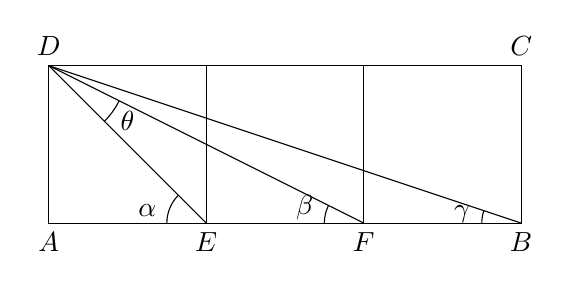
\begin{tikzpicture}
\draw (0,0)node[above]{$D$} rectangle (6,-2);
\draw (0,0) rectangle (4,-2);
\draw (0,0) rectangle (2,-2);
\foreach \x/\xtext in {0/A,2/E,4/F,6/B}
{
    \node at (\x,-2)[below]{$\xtext$};
}
\node at (6,0)[above]{$C$};

\foreach \x/\xtext in {2/45,4/26.56,6/18.43}
{
    \draw (\x-.5,-2) arc (180:180-\xtext:.5);
}

\foreach \x/\xtext in {2/\alpha,4/\beta,6/\gamma}
{
    \draw (0,0) --(\x,-2);
\node at (\x-.75,-2-.02*\x)[above]{$\xtext$};
}
\draw (360-45:1) arc (360-45:360-45+18.43:1);
\node at (1,-.7){$\theta$};
\end{tikzpicture}
    \caption{}
\end{figure}

\item 若$\sin\alpha=\frac{\sqrt{10}}{10}$, $\tan\beta=-\frac{1}{2}$. $90^{\circ}<\alpha<180^{\circ}$, $90^{\circ}<\beta<180^{\circ}$,求证:
\begin{enumerate}
    \item $\tan(\alpha+\beta)=-1$
    \item $\alpha+\beta=315^{\circ}$
\end{enumerate}

\item 已知$\cot\alpha=\frac{3}{4}$, $\cot\beta=\frac{1}{7}$,
且$\alpha,\beta$都是锐角,

求证:$1+\beta=135^{\circ}$。

\item 已知$\tan\alpha$与$\tan\beta$是方程$x^2+6x+7=0$的两个根。

求证:$\sin(\alpha+\beta) =\cos(\alpha+\beta)$

\item 已知 $a\cdot\sin(\theta+x)=b\sin(\theta+y)$, 求证:
\[\tan\theta=\frac{b\sin y-a\sin x}{a\cos x-b\cos y}\]

\end{enumerate}

\section{二倍角的正弦、余弦和正切}
\subsection{二倍角的正弦、余弦和正切}

在两角和的正弦、余
弦和正切的公式中,
令$\beta=\alpha$,则得到
\[\sin(\alpha+\alpha)=\sin\alpha\cos\alpha+\cos\alpha\sin\alpha\]
即
\begin{equation}
    \sin2\alpha=2\sin\alpha\cos\alpha
\end{equation}
\[\cos(\alpha+\alpha)=\cos\alpha\cos\alpha-\sin\alpha\sin\alpha\]
即
\begin{equation}
    \cos2\alpha=\cos^2\alpha-\sin^2\alpha
\end{equation}
若在公式(1.12)中,用$1-sin^2\alpha$代换 $\cos^2\alpha$, 或用$1-\cos^2\alpha$代换$\sin^2\alpha$, 则对于$\cos2\alpha$又得到两个公式
\begin{align}
    \cos2\alpha&=1-2\sin^2\alpha\\
    \cos2\alpha&=2\cos^2\alpha-1 
\end{align}
\[\tan (\alpha+\alpha)=\frac{\tan\alpha+\tan\alpha}{1-\tan\alpha\tan\alpha}\]
即:
\begin{equation}
    \tan2\alpha=\frac{2\tan\alpha}{1-\tan^2\alpha}
\end{equation}

\begin{rmk}
\begin{enumerate}
    \item 二倍角的三角函数的公式是把任意角的三角函数与小一半的角的三角函数联系起来,它们可以写成下面的各种形式的等式。例如
\[\begin{split}
    \sin4\alpha&=\sin2\cdot (2\alpha) =2\sin2\alpha\cos2\alpha\\
    \sin\alpha&=\sin2\left(\frac{\alpha}{2}\right)=2\sin\frac{\alpha}{2}\cos \frac{\alpha}{2}\\
    \cos\frac{\alpha}{2}&=\cos^2\frac{\alpha}{4}-\sin^2\frac{\alpha}{4}\\
    \tan3\alpha&=\frac{2\tan\frac{3\alpha}{2}}{1-\tan^2\frac{3\alpha}{2}}
\end{split}\]

\item 在二倍的正切公式(1.15)中,除了$\alpha=\frac{\pi}{2}+k\pi$和$\alpha=\frac{\pi}{4}+\frac{k\pi}{2},\; (k\in\mathbb{Z})$
诸值之外,对$\alpha$的其余一切值都成立,因为当所指定的那些$\alpha$值,$\tan\alpha$和$\tan2\alpha$都不存在。
\item 在使用二倍角三角函数的公式作恒等变形时,不仅要掌握从等式的左端的式子变换到右端的式子,而且也要熟练地掌握从等式的右端的式子变换到左端的式子。
\end{enumerate}
\end{rmk}

\begin{example}
    化简下面的式子
\begin{multicols}{2}
\begin{enumerate}
    \item $4\sin 15^{\circ}\cos 15^{\circ}$
    \item $\frac{1}{2}\sin 15^{\circ}\sin 255^{\circ}$
    \item $\cos^2\frac{\pi}{8}-\sin^2\frac{\pi}{8}$
    \item $\cos^2 15^{\circ}-\frac{1}{2}$
    \item $\frac{\tan 75^{\circ}}{1-\tan^2 75^{\circ}}$
\end{enumerate}
   \end{multicols} 
\end{example}

\begin{solution}
\begin{enumerate}
    \item $4\sin 15^{\circ}\cos 15^{\circ}=2\sin 30^{\circ}=1$
    \item $\frac{1}{2}\sin 15^{\circ}\sin 255^{\circ}=-\frac{1}{2}\sin 15^{\circ}\cos 15^{\circ}=-\frac{1}{4}\sin 30^{\circ}=-\frac{1}{8}$
    \item $\cos^2\frac{\pi}{8}-\sin^2\frac{\pi}{8}=\cos\frac{\pi}{4}=\frac{\sqrt{2}}{2}$
    \item $\cos^2 15^{\circ}-\frac{1}{2}=\frac{2\cos^2 15^{\circ}-1}{2}=\frac{\cos 30^{\circ}}{2}=\frac{\sqrt{3}}{4}$
    \item $\frac{\tan 75^{\circ}}{1-\tan^2 75^{\circ}}=\frac{1}{2}\frac{2\tan 75^{\circ}}{1-\tan^2 75^{\circ}}=\frac{1}{2}\tan 150^{\circ}=-\frac{1}{2}\tan 30^{\circ}=-\frac{\sqrt{3}}{6}$
\end{enumerate}    
\end{solution}

\begin{example}
    已知$0^{\circ}<\alpha<90^{\circ}$, $0^{\circ}<\beta<90^{\circ}$, $\tan\alpha=\frac{1}{7}$,
    $\sin\beta=\frac{1}{\sqrt{10}}$。
    
    求证:$\alpha+2\beta=45^{\circ}$
\end{example}

\begin{figure}[htp]
    \centering
        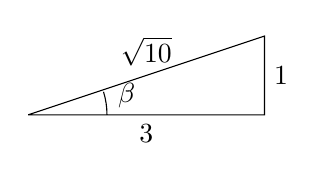
\begin{tikzpicture}
          \draw (0,0)--node[below]{3}(3,0)--node[right]{1}(3,1)--node[above]{$\sqrt{10}$}(0,0);
        \draw (1,0) arc (0:17:1);   
        \node at (1.25,.25){$\beta$};       
        \end{tikzpicture}
    \caption{}
\end{figure}


\begin{solution}
因为$\beta$是锐角,所以$\tan\beta=\frac{1}{3}$,由$\tan\beta<1$知$0^{\circ}<\beta<45^{\circ}$,同理$0^{\circ}<\alpha<45^{\circ}$。

又$\tan2\beta=\frac{\frac{2}{3}}{1-\left(\frac{1}{3}\right)^2}=\frac{3}{4}<1$

所以$0^{\circ}<2\beta <45^{\circ}$,并且
\[\tan(\alpha+2\beta)=\frac{\tan \alpha+\tan2\beta}{1-\tan \alpha\tan2\beta}=\frac{\frac{1}{7}+\frac{3}{4}}{1-\frac{1}{7}\cdot \frac{3}{4}}=1\]
所以$\alpha+2\beta=45^{\circ}+k\cdot 180^{\circ}\; (k\in\mathbb{Z})$,但是因为$0^{\circ}<\alpha<45^{\circ}$,$0^{\circ}<2\beta <45^{\circ}$,所以$0^{\circ}<\alpha+2\beta<90^{\circ}$,因此,$k$只能取0,因而:
\[\alpha+2\beta=45^{\circ}\]
\end{solution}


\begin{example}
用$\alpha$角的三角函数表示$\sin3\alpha$, $\cos3\alpha$和$\tan3\alpha$。
\end{example}



\begin{solution}
\begin{enumerate}
    \item \[\begin{split}
        \sin3\alpha&=\sin(\alpha+2\alpha)=\sin\alpha \cos2\alpha+\cos\alpha\sin2\alpha\\
        &=\sin\alpha(1-2\sin^2\alpha)+2\sin\alpha(1-\sin^2\alpha) \\
        &=\sin\alpha-2\sin^3\alpha+2\sin\alpha-2\sin^3\alpha\\
        &=3\sin\alpha-4\sin^3\alpha     
    \end{split}\]
    \item \[\begin{split}
       \cos3\alpha&=\cos(\alpha+2\alpha)=\cos\alpha\cos2\alpha-\sin\alpha\sin2\alpha\\
       &=\cos\alpha(2\cos^2\alpha-1)-2\cos\alpha(1-\cos^2\alpha)\\
       &=2\cos^3\alpha-\cos\alpha-2\cos\alpha+2\cos^3\alpha\\
       &=4\cos^3\alpha-3\cos\alpha 
    \end{split}\]
    \item \[\begin{split}
\tan3\alpha&=\tan(\alpha+2\alpha)=\frac{\tan\alpha+\tan2\alpha}{1-\tan\alpha\tan2\alpha}\\
&=\frac{\tan\alpha+\frac{2\tan\alpha}{1-\tan^2\alpha}}{1-\tan\alpha\cdot \frac{2\tan\alpha}{1-\tan^2\alpha}}\\
&=\frac{\tan\alpha-\tan^3\alpha+2\tan\alpha}{1-\tan^2\alpha-2\tan^2\alpha}\\
&=\frac{3\tan\alpha-\tan^3\alpha}{1-3\tan^2\alpha}        
    \end{split}\]
\end{enumerate}
\end{solution}

\begin{example}
求证:
\begin{enumerate}
    \item $[\sin\alpha(1-\sin\alpha)+\cos\alpha(1-\cos\alpha)]\x [\sin\alpha(1+\sin\alpha)+\cos\alpha(1+\cos\alpha)]=\sin2\alpha$
    \item $\sin 50^{\circ}\left(1+\sqrt{3}\tan 10^{\circ}\right)=1$
\end{enumerate}
\end{example}

\begin{proof}
\begin{enumerate}
    \item \[\begin{split}
 \text{左边}&=(\sin\alpha-\sin^2\alpha+\cos\alpha-\cos^2\alpha)\x (\sin\alpha+\sin^2\alpha+\cos\alpha+\cos^2\alpha)\\
 &=(\sin\alpha+\cos\alpha-1)(\sin\alpha+\cos\alpha+1)\\
 &=(\sin\alpha+\cos\alpha)^2-1\\
 &=2\sin\alpha\cos\alpha\\
 &=\sin2\alpha=\text{右边}       
    \end{split}\]
    \item \[\begin{split}
\text{左边}&= \sin 50^{\circ} \left(1+\frac{\sqrt{3}\sin 10^{\circ}}{\cos 10^{\circ}}\right)\\       
&= \sin 50^{\circ}\frac{2\left(\frac{1}{2}\cos10^{\circ}+\frac{\sqrt{3}}{2}\sin 10^{\circ}\right)}{\cos 10^{\circ}}\\
&=2\sin 50^{\circ}\cdot \frac{\cos60^{\circ}\cdot \cos10^{\circ}+\sin 60^{\circ}\cdot \sin 10^{\circ}}{\cos10^{\circ}}\\
&=\frac{2\sin50^{\circ}\cdot \cos50^{\circ}}{\cos10^{\circ}}\\
&=\frac{\sin100^{\circ}}{\cos10^{\circ}}\\
&=\frac{\cos10^{\circ}}{\cos10^{\circ}}=1=\text{右边}
    \end{split}\]
\end{enumerate}    
\end{proof}

\begin{ex}
\begin{enumerate}
    \item 不查表,求下列各式的值:
\begin{multicols}{2}
\begin{enumerate}
    \item $2\sin12^{\circ}30'\cdot \cos12^{\circ}30'$
    \item $\cos^2\frac{\pi}{12}-\sin^2\frac{\pi}{12}$
    \item $2\cos^2 67^{\circ}30'-1$
    \item $2\sin^2 75^{\circ}-1$
    \item $\frac{2\tan 22.5^{\circ}}{1-\tan^2 22.5^{\circ}}$
    \item $\sin 15^{\circ}\cdot \cos 15^{\circ}$
    \item $1-2\sin^2 750^{\circ}$
    \item $\frac{2\tan 150^{\circ}}{1-\tan^2 150^{\circ}}$
\end{enumerate}
\end{multicols}
\item 化简:
\begin{multicols}{2}
\begin{enumerate}
    \item $(\sin x-\cos y)^2$
    \item $\sin \frac{\alpha}{2}\cdot\cos\frac{\alpha}{2}$
    \item $\cos^4\theta-\sin^4\theta$
    \item $\frac{1}{1-\tan\theta}-\frac{1}{1+\tan\theta}$
\end{enumerate}
\end{multicols}

\item     已知$\cos\alpha=-\frac{12}{13},\; a\in \left(\frac{\pi}{2},\pi\right)$, 试求:$\sin2\alpha$, $\cos2\alpha$, $\tan2\alpha$的值。

\item 试推导出$\tan3\alpha$的公式(用$\tan\alpha$表示)。

\item 证明以下各等式:
\begin{enumerate}
    \item $\sin^2\theta=\frac{1}{2}(1-\cos2\theta)$
    \item $\cos^2\theta=\frac{1}{2}(1+\cos2\theta)$
    \item $2\sin(\pi+\alpha)\cos(\pi-\alpha)=\sin2\alpha$
    \item $\cos^4\frac{x}{2}-\sin^4\frac{x}{2}=\cos x$
    \item $1+2\cos^2\alpha=2+\cos2\alpha$
    \item $\frac{1}{\sin\alpha}-\frac{\cos2\alpha}{\sin\alpha}=2\sin\alpha$
    \item $\tan2\alpha=\frac{2\cot\alpha}{\cot^2\alpha-1}$
    \item $\frac{\sin^2\theta}{1-\cos^2\theta}=\cot\theta$
    \item $\cot x-\cot2x=\frac{1}{\sin 2x}$
    \item $\frac{\sin\beta\cdot \cos\beta}{\sin^2\beta-\cos^2\beta}=-\frac{1}{2}\tan2\beta$
\end{enumerate}
\end{enumerate}    


\end{ex}

\subsection{万能公式——用$\tan\frac{\alpha}{2}$分别表示任意角$\alpha$的三角函数}

\begin{blk}{定理}
若$\alpha\ne (2k+1)\pi\quad (k\in\mathbb{Z})$,则$\sin\alpha$, $\cos\alpha$和$\tan\alpha$可以表示成$\tan\frac{\alpha}{2}$的有理式,即:
\begin{align}
\sin\alpha &=\frac{2\tan\frac{\alpha}{2}}{1+\tan^2\frac{\alpha}{2}}\\
\cos\alpha&=\frac{1-\tan^2\frac{\alpha}{2}}{1+\tan^2\frac{\alpha}{2}}\\
\tan\alpha&=\frac{2\tan\frac{\alpha}{2}}{1-\tan^2\frac{\alpha}{2}}
\end{align}
\end{blk}

\begin{proof}
根据倍角公式有:
\[\begin{split}
    \sin\alpha &=2\sin\frac{\alpha}{2}\cos\frac{\alpha}{2}\\
    \cos\alpha &=\cos^2\frac{\alpha}{2}-\sin^2\frac{\alpha}{2}
\end{split}\]
或者
\[\sin\alpha=\frac{2\sin\frac{\alpha}{2}\cos\frac{\alpha}{2}}{\cos^2\frac{\alpha}{2}+\sin^2\frac{\alpha}{2}},\qquad \cos\alpha=\frac{\cos^2\frac{\alpha}{2}-\sin^2\frac{\alpha}{2}}{\cos^2\frac{\alpha}{2}+\sin^2\frac{\alpha}{2}}\]
上面两个等式的分母恒等于1, 因为$\alpha\ne \pi+2k\pi$,则$\frac{\alpha}{2}\ne \frac{\pi}{2}+k\pi\; (k\in\mathbb{Z})$, 因而$\cos\frac{\alpha}{2}\ne 0$。

上两式右边的分子、分母同除以$\cos^2\frac{\alpha}{2}\ne 0$, 得
\[\sin\alpha =\frac{2\tan\frac{\alpha}{2}}{1+\tan^2\frac{\alpha}{2}},\qquad
\cos\alpha=\frac{1-\tan^2\frac{\alpha}{2}}{1+\tan^2\frac{\alpha}{2}}\]
这两个式子相除就得到
\[\tan\alpha=\frac{2\tan\frac{\alpha}{2}}{1-\tan^2\frac{\alpha}{2}}\]
\end{proof}

上述三个公式通常叫做万能公式,应用它,就可以将$\alpha$角
的任一种三角函数化为以$\tan\frac{\alpha}{2}$为变量的有理函数,这对问题的解决往往是有益的。

\begin{example}
已知$\sin\alpha=0.8$, 且$90^{\circ}<\alpha<180^{\circ}$,
求$\sin2\alpha$, $cos2\alpha$

\end{example}

\begin{solution}
   除用倍角公式求解外,我们应用万能公式给出另解一种解法如下: 

因为$\sin\alpha=0.8,\; 90^{\circ}<\alpha<180^{\circ}$,所以$\tan\alpha=-\frac{4}{3}$
\[\begin{split}
    \sin2\alpha&=\frac{2\tan\alpha}{1+\tan^2\alpha}=\frac{-\frac{8}{3}}{1+\frac{16}{9}}=-\frac{24}{25} \\
    \cos2\alpha&=\frac{1-\tan^2\alpha}{1+\tan^2\alpha}=\frac{1-\left(-\frac{4}{3}\right)^2}{1+\left(\frac{4}{3}\right)^2}=-\frac{7}{25}
\end{split}  \]
\end{solution}


\begin{example}
已知$\cot\alpha=-2,\; 90^{\circ}<\alpha<180^{\circ}$, 

求$\sin2\alpha$, $\cos2\alpha$。
\end{example}

\begin{solution}
因为$\cot\alpha=-2,\; 90^{\circ}<\alpha<180^{\circ}$,所以$\tan\alpha=-\frac{1}{2}$
\[\begin{split}
    \sin2\alpha&=\frac{2\tan\alpha}{1+\tan^2\alpha}=\frac{2\left(-\frac{1}{2}\right)}{1+\left(-\frac{1}{2}\right)^2}=-\frac{4}{5} \\
    \cos2\alpha&=\frac{1-\tan^2\alpha}{1+\tan^2\alpha}=\frac{1-\frac{1}{4}}{1+\frac{1}{4}}=\frac{3}{5}
\end{split}  \]
\end{solution}



\begin{example}
    求证:$\frac{\cos A}{\cot \frac{A}{2}-\tan \frac{A}{2}}=\frac{1}{2}\sin A$
\end{example}

\begin{proof}
\[\begin{split}
\text{左边}&=\frac{\tan \frac{A}{2}\cdot \cos A}{1-\tan^2 \frac{A}{2}}\\
&=\frac{1}{2}\tan A\cdot \cos A\\
&=\frac{1}{2}\sin A=\text{右边}
  \end{split}\]  
\end{proof}

\begin{ex}
\begin{enumerate}
    \item 已知$\cos A=\frac{4}{5}$,且$\frac{3}{2}\pi<A<2\pi$,试用万能公式求$\tan\frac{A}{2}$.
    \item 应用万能公式求证:$\tan\frac{\pi}{8}=\sqrt{2}-1$
    \item 求证:
\begin{enumerate}
    \item $\frac{1}{4}\sin2\alpha=\frac{\cos^2\alpha    }{\cot\frac{\alpha}{2}-\tan\frac{\alpha}{2}}$
    \item $\frac{\sin 2x}{1+\cos2x}\cdot \frac{\cos x}{1+\cos x}=\tan\frac{x}{2}$
\end{enumerate}
\end{enumerate}
\end{ex}


\subsection{半角的正弦、余弦和正切}

用$\alpha$角的三角函数来
表示$\frac{\alpha}{2}$的角的三角函数的公式称为\textbf{半角三角函数公式}。在倍角公式:
\[\cos2\alpha=1-2\sin^2\alpha,\qquad \cos2\alpha=2\cos^2\alpha-1\]
里,用$\frac{\alpha}{2}$代替$\alpha$, 就得到
\[\cos\alpha=1-2\sin^2\frac{\alpha}{2},\qquad \cos\alpha=2\cos^2\frac{\alpha}{2}-1\]
所以
\[\sin^2\frac{\alpha}{2}=\frac{1-\cos\alpha}{2},\qquad \cos^2\frac{\alpha}{2}=\frac{1+\cos\alpha}{2}\]
由于$0\le \sin^2 \frac{\alpha}{2}\le 1$,
$0\le \cos^2\frac{\alpha}{2}\le 1$,故知
\[0\le \frac{1\pm\cos\alpha}{2}\le 1\]
两边开平方,得
\[\sin\frac{\alpha}{2}=\pm\sqrt{\frac{1-\cos\alpha}{2}},\qquad \cos\frac{\alpha}{2}=\pm\sqrt{\frac{1+\cos\alpha}{2}}\]
当$\alpha\ne(2k+1)\pi$时,$\cos\frac{\alpha}{2}\ne 0$且$\cos\alpha\ne -1$; 上面两个等式的两边相除,得到
\[\tan\frac{\alpha}{2}=\pm\sqrt{\frac{1-\cos\alpha}{1+\cos\alpha}}\]

下面三个公式称为半角的三角函数公式:
\begin{align}
    \sin\frac{\alpha}{2}&=\pm\sqrt{\frac{1-\cos\alpha}{2}}\\
     \cos\frac{\alpha}{2}&=\pm\sqrt{\frac{1+\cos\alpha}{2}}\\
     \tan\frac{\alpha}{2}&=\pm\sqrt{\frac{1-\cos\alpha}{1+\cos\alpha}}
\end{align}
其中:$\alpha\ne (2k+1)\pi$。
至于根号前正号或负号的选取是依半角的终边位于什么象限内而定。

\begin{example}
已知,$\cos\alpha=0.6$, $270^{\circ}<\alpha<360^{\circ}$

求$\sin \frac{\alpha}{2}$, $\cos\frac{\alpha}{2}$和$\tan \frac{\alpha}{2}$。
\end{example}

\begin{solution}
因为已知$270^{\circ}<\alpha<360^{\circ}$,所以$135^{\circ}<\frac{\alpha}{2}<180^{\circ}$
这时可以肯定$\frac{\alpha}{2}$角是第一象限的角,所以$\sin \frac{\alpha}{2}$的值是正的,$\cos\frac{\alpha}{2}$和$\tan \frac{\alpha}{2}$的值是负的,因此得到
\[\begin{split}
    \sin\frac{\alpha}{2}&=\sqrt{\frac{1-\cos\alpha}{2}}=\sqrt{\frac{1-0.6}{2}}=\frac{\sqrt{5}}{5}\\
     \cos\frac{\alpha}{2}&=-\sqrt{\frac{1+\cos\alpha}{2}}=-\sqrt{\frac{1+0.6}{2}}=-\frac{2\sqrt{5}}{5}\\
     \tan\frac{\alpha}{2}&=-\sqrt{\frac{1-\cos\alpha}{1+\cos\alpha}}=-\sqrt{\frac{1-0.6}{1+0.6}}=-\frac{1}{2}
\end{split}\]
\end{solution}

\begin{example}
    已知$\cos\alpha=-\frac{1}{3}$,求$\sin\frac{\alpha}{2}$。
\end{example}

\begin{solution}
因为$\cos\alpha=-\frac{1}{3}<0$, 所以$\alpha$角是第二或第三象限的角,即
\begin{equation}
    \frac{\pi}{2}+2k\pi<\alpha<\pi+2k\pi
\end{equation}
或者
\begin{equation}
    \pi+2k\pi<\alpha<\frac{3\pi}{2}+2k\pi\quad (k\in\mathbb{Z})
\end{equation}
从而由不等式(1.22)知道
\[\frac{\pi}{4}+k\pi<\frac{\alpha}{2}<\frac{\pi}{2}+k\pi \quad (k\in\mathbb{Z}) \]
当$k$为正、负偶数时,$\frac{\alpha}{2}$角是第一象限的角;当$k$为正、
负奇数时,$\frac{\alpha}{2}$角是第三象限的角,因此,尽管知道$\alpha$是第
二象限的角,也不能确定$\frac{\alpha}{2}$是第几象限的角,它可能是第一象限的角,也可能是第三象限的角,所以$\sin \frac{\alpha}{2}$的值取
符号“$+$”号或“$-$”号不能确定。

同理,由不等式(1.23)知道
\[\frac{\pi}{2}+k\pi<\frac{\alpha}{2}<\frac{3\pi}{4}+k\pi\quad (k\in\mathbb{Z})\]
当$k$为正负偶数时,
$\frac{\alpha}{2}$是第二象限角;当$k$为正负奇 数
时,$\frac{\alpha}{2}$是第二象限角,因此,当$\alpha$是第三象限的角时,$\frac{\alpha}{2}$
可能是第二象限的角或第四象限的角,所以$\sin\frac{\alpha}{2}$
的值的符号不能确定。

根据上面的讨论知道
\[\sin\frac{\alpha}{2}=\pm\sqrt{\frac{1-\cos\alpha}{2}}=\pm\sqrt{\frac{1+\frac{1}{3}}{2}}=\pm\frac{\sqrt{6}}{3}\]
\end{solution}

从上面的两个例子,可以知道,如果能确定$\alpha$角在哪
一个固定的区间,就可以确定角$\frac{\alpha}{2}$在哪一个固定的区间,这时公式(1.19)、(1.20)、(1.21)就能够选取固定的“$+$”号或“$-$”号;如果只知道角$\alpha$所在象限,而不知道它在哪一个固定的区间时,就不能确定角$\frac{\alpha}{2}$在哪一个固定的区间,这时公式(1.19)、(1.20)、(1.21)中,就应该保留“$\pm$”号。
    

\begin{example}
    利用半角公式求$\cos\frac{\pi}{8}$的值(准确到0.001)
\end{example}

\begin{solution}
    因为$\frac{\pi}{8}$是第一象限的角,把它作为$\frac{\pi}{4}$的半角,
    使得
\[\cos\frac{\pi}{8}=\sqrt{\frac{1+\cos\frac{\pi}{4}}{2}}=\sqrt{\frac{1+\frac{\sqrt{2}}{2}}{2}}=\frac{1}{2}\sqrt{2+\sqrt{2}}\approx 0.924\]
\end{solution}


\begin{example}
    求证:$\tan\frac{\alpha}{2}=\frac{\sin\alpha}{1+\cos\alpha}=\frac{1-\cos\alpha}{\sin\alpha}$
\end{example}
    
\begin{proof}
因为$\sin^2\alpha=1-\cos^2\alpha=(1+\cos \alpha)(1-\cos\alpha)$
,所以:
\[\frac{\sin\alpha}{1+\cos\alpha}=\frac{1-\cos\alpha}{\sin\alpha}\]
又$\tan\frac{\alpha}{2}=\frac{\sin\frac{\alpha}{2}}{\cos \frac{\alpha}{2}}=\frac{\sin\frac{\alpha}{2}\cdot 2\cos \frac{\alpha}{2}}{\cos\frac{\alpha}{2}\cdot 2\cos\frac{\alpha}{2}}=\frac{\sin\alpha}{1+\cos\alpha}$,因此:
\begin{equation}
    \tan\frac{\alpha}{2}=\frac{\sin\alpha}{1+\cos\alpha}=\frac{1-\cos\alpha}{\sin\alpha}
\end{equation}
\end{proof}

我们来说明,当$\alpha$是锐角时,这个公式的几何意义,如图1.4所示。
\begin{figure}[htp]
    \centering
\begin{tikzpicture}[>=latex, scale=1.4]
\draw[->] (-2,0)--(2,0)node[right]{$x$};
\draw[->] (0,-2)--(0,2)node[right]{$y$};    
\draw (0,0) circle (1.5);
\node at (-1.7,0)[below]{$B$};
\node at (1.7,0)[below]{$A$};
\node at (.2,-.2){$O$};
\draw[thick](0,0)--(60:1.5)node[above]{$P$}--(1.5/2,0)node[below]{$M$};
\draw[thick](-1.5,0)--(60:1.5);
\draw[->] (.5,0) arc(0:60:.5);
\draw[->] (-1.5,0)--+(.75,0) arc (0:30:.75);
\node at (.6,.2){$\alpha$};
\node at (-.6,.3){$\tfrac{\alpha}{2}$};

\end{tikzpicture}
    \caption{}
\end{figure}



在单位圆中,半径$|OA| = |OP| =|OB| =1$, $\angle POA=\alpha$ (弧度)。

于是,$\overline{MP}=\sin\alpha$, $\overline{OM}=\cos\alpha$, $\angle PBA=\frac{\alpha}{2}$
\[\tan\frac{\alpha}{2}=\frac{\overline{MP}}{\overline{BM}}=\frac{\overline{MP}}{\overline{BO}+\overline{OM}}=\frac{\sin\alpha}{1+\cos\alpha}\]

\begin{example}
求$\tan 15^{\circ}$的值。
\end{example}

\begin{solution}
解法1: $\tan 15^{\circ}=\frac{1-\cos30^{\circ}}{\sin 30^{\circ}}=\frac{1-\frac{\sqrt{3}}{2}}{\frac{1}{2}}=2-\sqrt{3}$

解法2: 
\[\begin{split}
  \tan 15^{\circ}&=\sqrt{\frac{1-\cos 30^{\circ}}{1+\cos 30^{\circ}}}=\sqrt{\frac{1-\frac{\sqrt{3}}{2}}{1+\frac{\sqrt{3}}{2}}}\\  
&=\sqrt{\frac{2-\sqrt{3}}{2+\sqrt{3}}}=\sqrt{(2-\sqrt{3})^2}\\
&=2-\sqrt{3}
\end{split}\]    
\end{solution}

由这两种解法看出,如果已知$\sin\alpha$, $\cos\alpha$的值,那么求$\tan\frac{\alpha}{2}$时,
用公式(1.24)要比公式(1.23)方便一些,其中尤
以$\tan\frac{\alpha}{2}=\frac{1-\cos\alpha}{\sin\alpha}$更方便。

\begin{example}
    求证:
\begin{multicols}{2}
    \begin{enumerate}
    \item $\tan\left(45^{\circ}-\frac{\alpha}{2}\right)=\frac{\cos\alpha}{1+\sin\alpha}$
    \item $\frac{\cos\alpha}{1-\sin\alpha}=\cot \left(45^{\circ}-\frac{\alpha}{2}\right)$
    \item $\frac{\cos^2 A}{\cot\frac{A}{2}-\tan\frac{A}{2}}=\frac{1}{4}\sin 2A$
\end{enumerate}
\end{multicols}
\end{example}

\begin{proof}
\begin{enumerate}
    \item \[\begin{split}
\tan\left(45^{\circ}-\frac{\alpha}{2}\right) &=\tan\frac{90^{\circ}-\alpha}{2}\\ 
&=\frac{\sin(90^{\circ}-\alpha)}{1+\cos(90^{\circ}-\alpha)}\\
&=\frac{\cos\alpha}{1+\sin\alpha}
    \end{split}\]

    \item \[\begin{split}
        \frac{\cos\alpha}{1-\sin\alpha}&= \frac{\sin(90^{\circ}-\alpha)}{1-\cos(90^{\circ}-\alpha)}\\
        &=\frac{1}{\tan\frac{90^{\circ}-\alpha}{2}}=\cot\frac{90^{\circ}-\alpha}{2}\\
&=\cot\left(45^{\circ}-\frac{\alpha}{2}\right)
    \end{split}\]

    \item \[\begin{split}
\frac{\cos^2 A}{\cot\frac{A}{2}-\tan\frac{A}{2}}&=\frac{\cos^2 A}{\frac{1+\cos A}{\sin A}-\frac{1-\cos A}{\sin A}}\\        
&=\frac{\sin A\cos^2 A}{2\cos A}\\
&=\frac{1}{2}\sin A\cdot \cos A\\
&=\frac{1}{4}\sin 2A
    \end{split}\]
\end{enumerate}    
\end{proof}

\begin{ex}
\begin{enumerate}
    \item 已知$\cos\alpha=\frac{2}{3}$,求$\sin\frac{\alpha}{2}$, $\cos \frac{\alpha}{2}$, $\tan \frac{\alpha}{2}$。
    \item 已知$\sin x=-\frac{4}{5}$,且$\frac{3\pi}{2}<x<2\pi$,求$\sin\frac{x}{2}$, $\cos \frac{x}{2}$, $\tan \frac{x}{2}$。
    \item 已知$\cos A=\frac{4}{5}$,且$A$是第四象限角,试求$\tan\frac{A}{2}$。
    \item 求证:
    \begin{multicols}{2}
\begin{enumerate}
    \item $\sin^2\frac{x}{4}=\frac{1-\cos\frac{x}{2}}{2}$
    \item $1+\sin\alpha=2\cos^2\left(\frac{\pi}{4}-\frac{\alpha}{2}\right)$
    \item $1-\sin\beta=2\cos^2\left(\frac{\pi}{4}+\frac{\beta}{2}\right)$
\item $\sin 4\alpha=\frac{4\sin\alpha(1-\tan^2\alpha)}{\sec\alpha(1+\tan^2\alpha)}$
\end{enumerate}        
    \end{multicols}
\end{enumerate}    
\end{ex}

\section*{习题1.2}
\addcontentsline{toc}{subsection}{习题1.2}
\begin{enumerate}
    \item 不查表计算下列的值
\begin{multicols}{2}
\begin{enumerate}
    \item $\sin 15^{\circ} \sin 75^{\circ}$
    \item $\sin \frac{\pi}{8} \sin \frac{3 \pi}{8}$
    \item $\frac{\tan\frac{\pi}{8}}{1-\tan^2\frac{\pi}{8}}$
    \item $\frac{1-\tan^2 15^{\circ}}{1+\tan^2 15^{\circ}}$
    \item $\cot\frac{\pi}{8}-\tan\frac{\pi}{8}$
    \item $\sin^{4} 105^{\circ}+\cos^{4} 75^{\circ}$
\end{enumerate}
\end{multicols}

\item 化简下面的式子
\begin{multicols}{2}
    \begin{enumerate}
        \item  $2-2 \sin ^{2} \alpha+\cos 2 \alpha$
        \item  $\cos 4 \alpha+2 \sin ^{2} 2 \alpha$
        \item $1-4 \sin ^{2} \alpha \cos ^{2} \alpha$
\item $\left(\cos ^{2} \alpha+2 \sin \alpha \cos \alpha-\sin ^{2} \alpha\right)^{2}$
\end{enumerate}
\end{multicols}

\item 证明:
\begin{enumerate}
    \item 若 $0<\alpha<\pi$, 则 $\sin 2 \alpha<2 \sin \alpha$
    \item 若 $0<\alpha<\frac{\pi}{4}$, 则 $\tan 2 \alpha<2\tan  \alpha$
\end{enumerate}

\item  已知 $\sin \alpha=\frac{7}{25}$, $\frac{\pi}{2}<\alpha<\pi$,
求 $\sin 2 \alpha$, $\cos 2 \alpha$ 和$\tan 2 \alpha$。

\item 已知$\cos\frac{\alpha}{2}=\frac{2n}{1+n^2}$,求$\sin\alpha$和$\tan\alpha$。
\item 已知$\sin\alpha=0.8$, $\cos\beta=-\frac{5}{13}$,并且
$\frac{\pi}{2}<\alpha<\pi$, $\frac{\pi}{2}<\beta<\pi$,求:
\begin{enumerate}
    \item $\sin(\alpha+2\beta)$
    \item $\cos(2\alpha-\beta)$
    \item $\tan[2(\alpha-\beta)]$
\end{enumerate}
\item 设方程$x^2-(\tan \theta+\cot \theta)x+1=0$的一个限是$2+\sqrt{3}$,
求$\sin2\theta$。
\item 设$\tan \theta$, $\tan \phi$是方程$7x^2+3x+1=0$的二根,
求 $\tan\frac{\theta+\phi}{2}$的值。
\item 若$\tan^2 \alpha-a\tan \alpha+1=0,\quad (a>0)$,
求$\cos2\alpha$。
\begin{enumerate}
    \item 当$0^{\circ}<\alpha<45^{\circ}$
    \item 当$45^{\circ}<\alpha<90^{\circ}$
\end{enumerate}

\item 如图1.5, 半径为$R$的圆木料,要截成横截面为长方形
的木料,问怎样截取,才可以使长方形截面的面积最大?
\begin{figure}[htp]
    \centering
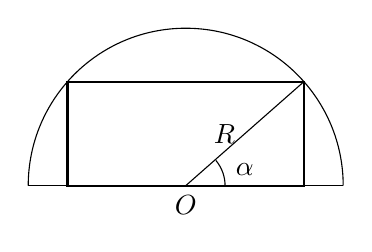
\begin{tikzpicture}
\draw (-2,0)--(2,0);
\draw (-2,0) arc (180:0:2);
\draw [thick] (-1.5,0) rectangle (1.5,1.32);
\draw (0,0)--node[left]{$R$}(1.5,1.32);
\node at (0,0)[below]{$O$};
\draw (.5,0) arc (0:40:.5);
\node at (.75,0)[above]{$\alpha$};

\end{tikzpicture}
    \caption{}
\end{figure}


\item 直角三角形的面积为12, 一锐角为$\beta$,求它的外接圆面
积,又当$\beta$是多少度时?外接圆面积最小。
\item 设 $\sin\alpha +\cos\alpha=\frac{1}{5}$,
求 $\sin2\alpha$, $\sin\alpha$, $\cos\alpha$, $\cos \frac{\alpha}{2}$, $\sin \frac{\alpha}{2}$。

\item \begin{enumerate}
    \item 已知$\cos\alpha =\frac{119}{169}$,求$\sin\frac{\alpha}{2}$, $\cos\frac{\alpha}{2}$和$\tan\frac{\alpha}{2}$。
    \item 已知$\cos\phi=\frac{1}{3}$,且$\phi\in(270^{\circ}, 360^{\circ})$,求$\sin\frac{\phi}{2}$, $\cos\frac{\phi}{2}$及$\tan\frac{\phi}{2}$。
\end{enumerate}
\item 已知$\cos\alpha=\frac{4}{5}$,且$\frac{3\pi}{2}<\alpha<2\pi$,求$\tan\frac{\alpha}{2}$。
\item 已知,等腰三角形顶角的余弦等于$\frac{7}{25}$, 求底角的正弦、
余弦和正切。
\item \begin{enumerate}
    \item 已知$\tan\alpha=\frac{4}{5}$, $180^{\circ}<\alpha<270^{\circ}$。
求$\tan\frac{\alpha}{2}$, $\sin2\alpha$, $\cos2\alpha$, $\tan 2\alpha$。
\item 已知$2\sin x+3\cos x=2$, 
求$\sin x$ 和 $\cos x$的值。
\end{enumerate}

\item 求证:
\begin{enumerate}
    \item $\left(\sin\frac{x}{2}-\cos\frac{x}{2}\right)^2=1-\sin x$
    \item $\tan\alpha-\cot\alpha=-2\cot 2\alpha$
    \item $\tan\left(\alpha+\frac{\pi}{4}\right)+\tan\left(\alpha-\frac{\pi}{4}\right)=2\tan\alpha$
    \item $\sin\theta+\cos\theta=\frac{1+\sin2\theta}{\sin\theta+\cos\theta}$
    \item $\sin\alpha(1+\cos2\alpha)=\sin2\alpha\cdot \cos\alpha$
    \item $2\sin\left(\frac{\pi}{4}+x\right)\sin\left(\frac{\pi}{4}-x\right)=\cos2x$
    \item $\frac{1+\tan\alpha}{1-\tan\alpha}=\frac{1+\sin2\alpha}{\cos^2\alpha-\sin^2\alpha}$
    \item $\frac{1+\sin2\theta-\cos2\theta}{1+\sin2\theta+\cos2\theta}=\tan\theta$
    \item $\frac{2\sin x-\sin2x}{2\sin x+\sin2x}=\tan^2\frac{x}{2}$
    \item $\frac{\tan\frac{\alpha}{2}}{1+\tan\frac{\alpha}{2}}+\frac{\tan\frac{\alpha}{2}}{1-\tan\frac{\alpha}{2}}=\tan\alpha$
\end{enumerate}

\item 利用$45^{\circ}$, $30^{\circ}$的三角函数值,求$\cos22^{\circ}30'$; $\sin22^{\circ}30'$; $\cos15^{\circ}$, $\sin15^{\circ}$的值。
\item \begin{enumerate}
    \item 求$\sin18^{\circ}$的值;
    \item 求证$\cos36^{\circ}-\cos72^{\circ}=\frac{1}{2}$。
\end{enumerate}

\item 求证:
\begin{enumerate}
    \item $\sin\frac{\pi}{8}=\frac{1}{2}\sqrt{2-\sqrt{2}}$
    \item $\tan 67.5^{\circ}=\sqrt{2}+1$
    \item $\tan 7^{\circ}30'=\sqrt{6}-\sqrt{3}+\sqrt{2}-2$
\end{enumerate}
\item 证明下列恒等式
\begin{enumerate}
    \item $2\sin\theta+\sin2\theta=4\sin\theta\cdot \cos^2\frac{\theta}{2}$
    \item $\tan 15^{\circ}+\cot 15^{\circ}=4$
    \item $\cos^2\alpha-2=\cos2\alpha\cdot \csc^2\alpha$
    \item $\sin(n\pi+x)\cos(n\pi-x)=\frac{1}{2}\sin 2x,\quad (n\in \mathbb{Z})$
    \item $\cos\alpha(\cos\alpha-\cos\beta)+\sin\alpha(\sin\alpha-\sin\beta)=2\sin^2\frac{\alpha-\beta}{2}$
    \item $\frac{\cos\alpha}{\sec\frac{\alpha}{2}+\csc\frac{\alpha}{2}}=\frac{1}{2}\left(\cos\frac{\alpha}{2}-\sin\frac{\alpha}{2}\right)$
    \item $\cos^4\theta=\frac{1}{4}+\frac{1}{2}\cos2\theta+\frac{1}{4}\cos^2 2\theta$
    \item $\sin^4\theta=\frac{3}{8}-\frac{1}{2}\cos2\theta+\frac{1}{8}\cos4\theta$
\end{enumerate}

\item 求证下列条件等式:
\begin{enumerate}
    \item 若$\tan x=\frac{b}{a}$,则$a\cos 2x+b\sin 2x=a$
    \item 若$\tan\alpha\frac{\alpha}{2}=\frac{m}{n}$,则$\sin\alpha+\frac{m}{n}\cos\alpha=1$
    \item 若$1+2\tan^2 x=\tan^2 y$,则$\sin^2x+\cos 2y=0$
    \item 若$x+y=3-\cos4\alpha$, $x-y=4\sin2\alpha$,则$x^{\tfrac{1}{2}}+y^{\tfrac{1}{2}}=2$
    \item 若$2\alpha+\beta=\frac{\pi}{2}$,则
    \[\sin\alpha=\sqrt{\frac{1-\sin\beta}{2}},\qquad \cos\alpha=\sqrt{\frac{1+\sin\beta}{2}}\]
\end{enumerate}
\end{enumerate}

\section{三角函数的和差化积与积化和差}
\subsection{三角函数的和差化积}

根据两角和差的正弦函数的定理有:
\[\begin{split}
    \sin(x+y)&=\sin x\cos y+\cos x\sin y\\
    \sin(x-y)&=\sin x\cos y-\cos x\sin y\\
\end{split}\]

由这两个等式左、右两端相加和相减得:
\begin{align}
 \sin (x+y) +\sin (x-y) &=2\sin x\cos y\\
\sin (x+y)-\sin (x-y) &=2\cos x\sin y   
\end{align}
设$x+y=\alpha$, $x-y=\beta$, 那么
\begin{equation}
    x=\frac{\alpha+\beta}{2},\qquad y=\frac{\alpha-\beta}{2}
\end{equation}

因此,上面两个等式(1.25)和(1.26)就变成
\begin{align*}
\sin\alpha+\sin\beta&=2\sin\frac{\alpha+\beta}{2}\cos\frac{\alpha-\beta}{2}\tag{I}\\
\sin\alpha-\sin\beta&=2\cos\frac{\alpha+\beta}{2}\sin\frac{\alpha-\beta}{2}\tag{II}
\end{align*}
根据两角和差的余弦函数的定理有:
\[\begin{split}
    \cos (x+y) &=\cos x\cos y - \sin x\sin y\\
\cos (x-y) &=\cos x\cos y +\sin x \sin y
\end{split}\]
由这两个等式左、右两端相加和相减得:
\begin{align}
    \cos (x+y) +\cos(x-y)&=2\cos x\cos y\\
\cos (x+y) -\cos (x-y) &=-2\sin x\sin y
\end{align}
以等式(1.27)代入上式得:
\begin{align*}
\cos\alpha+\cos\beta&=2\cos\frac{\alpha+\beta}{2}\cos\frac{\alpha-\beta}{2}\tag{III}\\
\cos\alpha-\cos\beta&=-2\sin\frac{\alpha+\beta}{2}\sin\frac{\alpha-\beta}{2}\tag{IV}
\end{align*}

利用上面得到的四个公式;即
\begin{blk}{和差化积公式}
\begin{align*}
    \sin\alpha+\sin\beta&=2\sin\frac{\alpha+\beta}{2}\cos\frac{\alpha-\beta}{2}\tag{I}\\
\sin\alpha-\sin\beta&=2\cos\frac{\alpha+\beta}{2}\sin\frac{\alpha-\beta}{2}\tag{II}\\
\cos\alpha+\cos\beta&=2\cos\frac{\alpha+\beta}{2}\cos\frac{\alpha-\beta}{2}\tag{III}\\
\cos\alpha-\cos\beta&=-2\sin\frac{\alpha+\beta}{2}\sin\frac{\alpha-\beta}{2}\tag{IV}
\end{align*}
\end{blk}

可以把某些三角函数的和或差化成积的形式。


\begin{example}
    把下列各式化成积的形式
\begin{multicols}{2}
\begin{enumerate}
    \item $1+\sin\alpha$
    \item $1-2\sin\alpha$
    \item $\sin\frac{\pi}{5}+\cos\frac{\pi}{5}$
    \item $\cos22^{\circ}-\sin 66^{\circ}$
\end{enumerate}
\end{multicols}
\end{example}

\begin{solution}
\begin{enumerate}
    \item 方法1: 
\[\begin{split}
    1+\sin\alpha&=\sin90^{\circ}+\sin\alpha\\
    &=2\sin\frac{90^{\circ}+\alpha}{2}\cos\frac{90^{\circ}-\alpha}{2}\\
    &=2\sin\left(45^{\circ}+\frac{\alpha}{2}\right)\cos\left(45^{\circ}-\frac{\alpha}{2}\right)\\
    &=2\sin^2\left(45^{\circ}+\frac{\alpha}{2}\right)=2\cos^2\left(45^{\circ}-\frac{\alpha}{2}\right)
\end{split}\]

方法2: 
\[\begin{split}
    1+\sin\alpha &=1+\cos(90^{\circ}-\alpha)\\
    &=2\cos^2\left(45^{\circ}-\frac{\alpha}{2}\right)
\end{split}\]
\item \[\begin{split}
    1-2\sin\alpha &=2\left(\frac{1}{2}-\sin\alpha\right)\\
    &=2(\sin30^{\circ}-\sin\alpha)\\
    &=2\x 2\cos\frac{30^{\circ}+\alpha}{2}\sin\frac{30^{\circ}-\alpha}{2}\\
    &=4\cos\left(15^{\circ}+\frac{\alpha}{2}\right)\sin \left(15^{\circ}-\frac{\alpha}{2}\right)
\end{split}\]    
\item \[\begin{split}
    \sin\frac{\pi}{5}+\cos\frac{\pi}{5}&= \cos\left(\frac{\pi}{2}-\frac{\pi}{5}\right)+\cos\frac{\pi}{5}\\
    &=\cos\frac{3\pi}{10}+\cos\frac{\pi}{5}\\
    &=2\cos\frac{\frac{3\pi}{10}+\frac{2\pi}{10}}{2}\cos\frac{\frac{3\pi}{10}-\frac{2\pi}{10}}{2} \\
    &=2\cos\frac{\pi}{4}\cos\frac{\pi}{20}\\
    &=\sqrt{2}\cos\frac{\pi}{20}
\end{split}\]    
\item \[\begin{split}
    \cos22^{\circ}-\sin 66^{\circ}&=\cos22^{\circ}-\cos(90^{\circ}-66^{\circ}) \\
    &=\cos22^{\circ}-\cos 24^{\circ}\\
    &=-2\sin\frac{46^{\circ}}{2}\sin\left(-\frac{2^{\circ}}{2}\right)\\
    &=2\sin 23^{\circ}\sin 1^{\circ}
\end{split}\]    
\end{enumerate}
\end{solution}


\begin{example}
    把$\sin^2\alpha-\sin^2\beta$化为乘积形式。
\end{example}

\begin{solution}
方法1:
\[\begin{split}
    \sin^2\alpha-\sin^2\beta&=(\sin\alpha+\sin\beta)(\sin\alpha-\sin\beta)\\
    &=\left(2\sin\frac{\alpha+\beta}{2}\cos\frac{\alpha-\beta}{2}\right)\left(2\cos\frac{\alpha+\beta}{2}\sin\frac{\alpha-\beta}{2}\right)\\
    &=\left(2\sin\frac{\alpha+\beta}{2}\cos\frac{\alpha+\beta}{2}\right)\left(2\sin\frac{\alpha-\beta}{2}\cos\frac{\alpha-\beta}{2}\right)\\
    &=\sin(\alpha+\beta)\sin(\alpha-\beta)
\end{split}\]

方法2: 利用公式$\sin^2\alpha=\frac{1-\cos2\alpha}{2}$
进行替换,得到
\[\begin{split}
    \sin^2\alpha-\sin^2\beta&=\frac{1-\cos2\alpha}{2}-\frac{1-\cos2\beta}{2}\\
    &=\frac{1}{2}(\cos2\beta-\cos2\alpha)\\
    &=\frac{1}{2}\x (-2)\sin(\beta+\alpha)\sin(\beta-\alpha)\\
    &=\sin(\alpha+\beta)\sin(\alpha-\beta)
\end{split}\]
\end{solution}


\begin{example}
    引入辅助角把下面各式化为两角和的正弦函数。
\begin{enumerate}
    \item $3\cos\alpha+\sqrt{3}\sin\alpha$
    \item $3\cos\alpha-\sqrt{3}\sin\alpha$
    \item $\cos 2x-4\sin 2x$
\end{enumerate}
\end{example}

\begin{solution}
\begin{enumerate}
    \item \[\begin{split}
3\cos\alpha+\sqrt{3}\sin\alpha &=\sqrt{3}\left(\sqrt{3}\cos\alpha+\sin\alpha\right)\\
&=2\sqrt{3}\left(\frac{\sqrt{3}}{2}\cos\alpha+\frac{1}{2}\sin\alpha\right)\\
&=2\sqrt{3}\left(\sin60^{\circ}\cos\alpha+\cos60^{\circ}\sin\alpha\right)\\
&=2\sqrt{3}\sin(60^{\circ}+\alpha)=2\sqrt{3}\sin (\alpha+60^{\circ})        
    \end{split}\]

    \begin{figure}[htp]
        \centering
    \begin{tikzpicture}[>=latex]
\draw[->] (-2,0)--(2,0)node[right]{$x$};
\draw[->] (0,-2)--(0,2)node[right]{$y$};    
\draw[<->] (-1.1,0)--node[fill=white]{$\tfrac{\sqrt{3}}{2}$}(-1.1,1.3);
    \node at (.2,-.2){$O$};
\draw[thick] (0,0)--(120:1.5)--(-.75,0)node[below]{$-\tfrac{1}{2}$};
\draw[->] (.5,0) arc (0:120:.5);
\node at (60:.5)[right]{$120^{\circ}$};
\draw (120:1.5)--+(-.5,0);
\draw (0,0) circle(1.5) ; 
    \end{tikzpicture}
        \caption{}
    \end{figure}

    \item \[\begin{split}
 3\cos\alpha-\sqrt{3}\sin\alpha&=2\sqrt{3}\left(\frac{\sqrt{3}}{2}\cos\alpha-\frac{1}{2}\sin\alpha\right)\\       
 &=2\sqrt{3}\left(\sin120^{\circ}\cos\alpha+\cos120^{\circ}\sin\alpha\right)\\
 &=2\sqrt{3}\sin(120^{\circ}+\alpha)=2\sqrt{3}\sin (\alpha+120^{\circ})      
    \end{split}\]
    \item 配一个正系数$k$,使得
\[\cos 2x-4\sin 2x=k\left(\frac{1}{k}\cos2x-\frac{4}{k}\sin 2x\right)\]    
    并且引入一个辅助角$\theta$,满足下面两个等式:
\[\sin\theta=\frac{1}{k},\qquad \cos\theta=-\frac{4}{k}\]
$k$的值可由等式$\sin^2\theta+\cos^2\theta=\frac{1+(-4)^2}{k^2}=1$确定,于是有:
\[k=\sqrt{1+16}=\sqrt{17}\]
于是$\sin\theta=\frac{1}{\sqrt{17}}$, $\cos\theta=-\frac{4}{\sqrt{17}}$。$\theta$是第二象限角,它的值可由$\tan\theta=-\frac{1}{4}=-0.25$求出,得到
\[\theta=180^{\circ}-14^{\circ}2'=165^{\circ}58'\]
因此:
    \[\begin{split}
 \cos 2x-4\sin 2x&=\sqrt{17}\left(\sin165^{\circ}58'\cos 2x+\cos165^{\circ}58'\sin2x \right)       \\
 &=\sqrt{17}\sin (2x+165^{\circ}58')
    \end{split}\]
\end{enumerate}     
\end{solution}

\begin{example}
    化$a\sin x+b\cos x$为积的形式。
\end{example}

\begin{analyze}
仿照例1.29可以引入一个辅助角$\theta$, 并配上一个
正系数$k$, 我们来分析如何确定$k,\theta$:

假设$a=k\cdot \cos\theta$, $b=k\cdot\sin\theta$, 原式就变为
\[\begin{split}
    a\sin x+b\cos x&=k(\sin x\cdot \cos\theta+ \cos x\cdot \sin\theta)\\
    &=k\cdot \sin (x+\theta) 
\end{split}\]

由于$\sin^2\theta+\cos^2\theta=1$, 因而$\left(\frac{a}{k}\right)^2+\left(\frac{b}{k}\right)^2=1$
\[\therefore\quad k=\sqrt{a^2+b^2}\]
于是就得出
\[\cos\theta=\frac{a}{\sqrt{a^2+b^2}},\qquad  \sin\theta=\frac{b}{\sqrt{a^2+b^2}} \]
从而得
\[\tan\theta =\frac{b}{a}\]
这样,由$a,b$就可以确定$k,\theta$的值了。
\end{analyze}

\begin{solution}
\[a\sin x+b\cos x=\sqrt{a^2+b^2}\left(\frac{a}{\sqrt{a^2+b^2}}\sin x+\frac{b}{\sqrt{a^2+b^2}}\cos x\right)\]
令$\cos\theta=\frac{a}{\sqrt{a^2+b^2}},\quad  \sin\theta=\frac{b}{\sqrt{a^2+b^2}}$,则
\[\begin{split}
    \text{原式}&=\sqrt{a^2+b^2}(\cos\theta\cdot \sin x+\sin\theta \cdot \cos x)\\
&=\sqrt{a^2+b^2}\sin (x+\theta)
\end{split}\]
其中,$\theta$角所在的象限由$a,b$的符号确定,$\theta$角的值由
$\tan\theta=\frac{b}{a}$确定。
\end{solution}


\begin{example}
    若$A+B+C=180^{\circ}$, 求证
$\sin2A+\sin2B+\sin2C=4\sin A\sin B\sin C$
\end{example}

\begin{proof}
\begin{align*}
  &\quad   \sin2A+\sin2B+\sin2C\\
    &=2\sin (A+B) \cos(A-B) +2\sin C\cos C\\
    &=2\sin C\cos (A-B) +2\sin C\cos C \tag{$\sin (A+B)=\sin C$}\\
    &=2\sin C [\cos(A-B)+\cos C]\\
    &=2\sin C [\cos(A-B)-\cos(A+B)]
    \tag{$\cos C=-\cos (A+B)$}\\
    &=2\sin C [-2\sin A\sin (-B)]\\
    &=4\sin A\sin B\sin C  
\end{align*}
\end{proof}

\begin{rmk}
    在证明满足条件$A+B+C=180^{\circ}$ 的三个角$A$、$B$、$C$的三角函数恒等式时,要特别注意互为余角与互为补角的三角函数的性质,例如:    
从任何两个角的和是第三个角的补角这一类关系,得到
\[\sin (B+C) =\sin A,\qquad  \cos (A+B) = - \cos C,\qquad \tan (C+A) =-\tan B\]
\[\cos B= -\cos (C+A),\qquad \sin C=\sin (A+B) ,\qquad  \cot A=-\cot (B+C)\]

又从任何两个角的和的一半是第三个角的一半的余角这
一关系得到
\[\cos\frac{A+B}{2}=\sin\frac{C}{2},\qquad \sin\frac{C+A}{2}=\cos\frac{B}{2},\qquad \tan\frac{B+C}{2}=\cot\frac{A}{2}\]
\[\cos\frac{C}{2}=\sin\frac{A+B}{2},\qquad \sin\frac{A}{2}=\cos\frac{B+C}{2},\qquad \tan\frac{B}{2}=\cot\frac{C+A}{2}\]
\end{rmk}


\begin{example}
    把$1+\sin\theta+\cos\theta$化成积的形式。
\end{example}

\begin{solution}
\[\begin{split}
1+\sin\theta+\cos\theta&=(1+\cos\theta)+\sin\theta\\
&=2\cos^2\frac{\theta}{2}+2\sin\frac{\theta}{2}\cdot \cos\frac{\theta}{2}\\
&=2\cos\frac{\theta}{2}\left(\cos\frac{\theta}{2}+\sin\frac{\theta}{2}\right)\\
&=2\cos\frac{\theta}{2}\left[\sin\left(90^{\circ}-\frac{\theta}{2}\right)+\sin \frac{\theta}{2}\right]\\
&=2\cos\frac{\theta}{2}\cdot 2\sin 45^{\circ}\cdot \cos\left(45^{\circ}-\frac{\theta}{2}\right)\\
&=2\sqrt{2}\cos \frac{\theta}{2}\cdot \cos\left(45^{\circ}-\frac{\theta}{2}\right)
\end{split}\]
\end{solution}

\begin{ex}
\begin{enumerate}
    \item 把下列各式化为积的形式(口答)
\begin{multicols}{2}
\begin{enumerate}
    \item $\sin 24^{\circ}+\sin 20^{\circ}$
    \item $\sin 75^{\circ}-\sin 15^{\circ}$
    \item $\cos 3x+\cos 2x$
    \item $\cos\frac{\alpha+\beta}{2}-\cos\frac{\alpha-\beta}{2}$
\end{enumerate}
\end{multicols}

\item 求值:
\begin{enumerate}
    \item $\frac{\sin20^{\circ}-\sin 40^{\circ}}{\cos 20^{\circ}-\sin 40^{\circ}}$
    \item $\sin 20^{\circ}+\sin 40^{\circ}-\sin 80^{\circ}$
\end{enumerate}

\item 求证:
\begin{enumerate}
    \item $\frac{\sin\alpha+\sin\beta}{\sin\alpha-\sin\beta}=\tan\frac{\alpha+\beta}{2}\cdot \cot\frac{\alpha-\beta}{2}$
    \item $\frac{\sin x+\sin y}{\cos x-\cos y}=\cot\frac{y-x}{2}$
    \item $\cos 2A+\cos 2B+\cos 2C=-1-4\cos A\cdot \cos B\cdot \cos C$,其中$A+B+C=\pi$
\end{enumerate}

\item 将下列各式化为两角和(差)的三角函数:
\begin{multicols}{2}
\begin{enumerate}
    \item $\frac{\sqrt{3}}{2}\sin x+\frac{1}{2}\sin x$
    \item $\frac{\sqrt{2}}{2}\cos x-\frac{\sqrt{2}}{2}\sin x$
    \item $\sqrt{2}\cos x+\sqrt{2}\sin x$
    \item $\cos\theta-\sqrt{3}\sin\theta$
    \item $4\sin\alpha+3\cos\alpha$
    \item $3\cos\beta-\sqrt{7}\sin\beta$
\end{enumerate}
\end{multicols}
\end{enumerate}
\end{ex}

\subsection{三角函数的积化和差}
将公式(1.25)、(1.26)、(1.28)、(1.29)的两边同除以2,便得到如下公式:

\begin{blk}{积化和差公式}
\begin{align*}
\sin x\cdot\cos y  &= \frac{1}{2} [\sin (x+y) +\sin (x-y)] \tag{V}\\
\cos x\cdot \sin y &=\frac{1}{2}  [\sin (x+y)-\sin (x-y)] \tag{VI} 
\end{align*} 
\begin{align*}
\cos x\cdot\cos y  &= \frac{1}{2} [\cos (x+y) +\cos (x-y)] \tag{VII}\\
\cos x\cdot \sin y &=-\frac{1}{2}  [\cos (x+y)-\cos (x-y)]  \\
&=\frac{1}{2}[\cos (x-y)-\cos (x+y)] \tag{VIII}
\end{align*} 
\end{blk}

若$x=y$,由此可推出倍角公式,即有
\[\sin x\cos x=\frac{1}{2}\sin 2x,\qquad \cos^2 x=\frac{1}{2}(1+\cos 2x),\qquad \sin^2x=\frac{1}{2}(1-\cos2x)\]

\begin{example}
    化乘积$\sin35^{\circ} \cos55^{\circ}$ 为和的形式。
\end{example}

\begin{solution}
解法1: 
\[\sin35^{\circ} \cos55^{\circ} =\frac{1}{2}[\sin90^{\circ} +\sin (-20^{\circ} ) ]
=\frac{1}{2} [1-\sin20^{\circ} ]\]

解法2:
\[\sin35^{\circ} \cos55^{\circ}=\sin^2 35^{\circ} =\frac{1-\cos 70^{\circ}}{2}=\frac{1-\sin 20^{\circ}}{2}\]
\end{solution}


\begin{example}
    不查表,求下列各式的值:
\begin{enumerate}
    \item $\sin\frac{5\pi}{12}\cdot\cos\frac{\pi}{12}$
    \item $\cos^2 73^{\circ} +\cos^2 47^{\circ} +\cos73^{\circ} \cos47^{\circ}$
\end{enumerate}
\end{example}

\begin{solution}
\begin{enumerate}
    \item 解法1: 
\[\begin{split}
    \sin\frac{5\pi}{12}\cdot\cos\frac{\pi}{12}&=\frac{1}{2}\left[\sin\frac{\pi}{2}+\sin\frac{\pi}{3}\right]\\
    &=\frac{1}{2}+\frac{\sqrt{3}}{4}=\frac{1}{4}(2+\sqrt{3})
\end{split}\]    

解法2: 
\[\begin{split}
    \sin\frac{5\pi}{12}\cdot\cos\frac{\pi}{12}&=\cos\frac{\pi}{12}\cdot \cos\frac{\pi}{12}\\
    &=\cos^2\frac{\pi}{12}=\frac{1}{2}\left(1+\cos\frac{\pi}{6}\right)\\
    &=\frac{1}{2}\left(1+\frac{\sqrt{3}}{2}\right)=\frac{1}{4}\left(2+\sqrt{3}\right)
\end{split}\]    

\item \[\begin{split}
    \text{原式}&=1+\frac{\cos146^{\circ}}{2}+\frac{1+\cos94^{\circ}}{2}+\frac{\cos120^{\circ}+\cos26^{\circ}}{2}\\
    &=1+\frac{\cos146^{\circ}+\cos94^{\circ}}{2}-\frac{1}{4}+\frac{\cos26^{\circ}}{2}\\
    &=\frac{3}{4}+\frac{2\cos120^{\circ}\cos26^{\circ}}{2}+\frac{\cos26^{\circ}}{2}\\
    &=\frac{3}{4}-\frac{\cos26^{\circ}}{2}+\frac{\cos26^{\circ}}{2}\\
    &=\frac{3}{4}
\end{split}\]
\end{enumerate}
\end{solution}


\begin{example}
化简$\cos\alpha\cdot \cos2\alpha\cdot \cos4\alpha$并求$\cos\frac{\pi}{7}\cos\frac{2\pi}{7}\cos\frac{4\pi}{7}$的值。
\end{example}

\begin{solution}
\[\begin{split}
    \cos\alpha\cdot \cos2\alpha\cdot \cos4\alpha&=\frac{2\sin\alpha\cdot \cos\alpha\cdot \cos2\alpha\cdot \cos4\alpha}{2\sin\alpha}\\
    &=\frac{\sin2\alpha\cdot \cos2\alpha\cdot \cos4\alpha}{2\sin\alpha}\\
    &=\frac{\sin4\alpha\cdot \cos4\alpha}{2^2\sin\alpha}\\
    &=\frac{\sin8\alpha}{2^3\sin\alpha}=\frac{\sin 8\alpha}{8\sin \alpha}
\end{split}
\]
\[\cos\frac{\pi}{7}\cos\frac{2\pi}{7}\cos\frac{4\pi}{7}=\frac{\sin \frac{8\pi}{7}}{8\sin \frac{\pi}{7}}=\frac{-\sin\frac{\pi}{7}}{8\sin\frac{\pi}{7}}=-\frac{1}{8}\]
    
\end{solution}

\begin{example}
求证:
\begin{enumerate}
    \item $\sin15^{\circ} \cdot \sin30^{\circ} \cdot \sin75^{\circ} =\frac{1}{8}$
   \item  $\cos10^{\circ} \cdot \cos30^{\circ} \cdot \cos50^{\circ} \cdot \cos70^{\circ} =\frac{3}{16}$
\end{enumerate}    
\end{example}

\begin{proof}
\begin{enumerate}
    \item 证法1:
\[\begin{split}
\text{左边}&=\frac{1}{2}\sin 15^{\circ}\cdot \sin 75^{\circ}\\
&=-\frac{1}{4}[\cos 90^{\circ}-\cos(-60^{\circ})]\\
&=-\frac{1}{4}(0-\cos60^{\circ})\\
&=-\frac{1}{4}\left(-\frac{1}{2}\right)=\frac{1}{8}=\text{右边}    
\end{split}\]

证法2:
\[\begin{split}
\text{左边}&=\frac{1}{2}\sin 15^{\circ}\cdot \sin 75^{\circ}\\
&=\frac{1}{2}\sin 15^{\circ}\cdot \cos15^{\circ}\\
&=\frac{1}{4}\sin 30^{\circ}=\frac{1}{8}=\text{右边}    
\end{split}\]

\item 
\[\begin{split}
\text{左边}&=\cos 10^{\circ}\cdot \frac{\sqrt{3}}{2}\cdot \frac{1}{2}[\cos 120^{\circ}+\cos(-20^{\circ})]\\
&=\frac{\sqrt{3}}{4}\cos 10^{\circ}\left(-\frac{1}{2}+\cos20^{\circ}\right)\\ 
&=-\frac{\sqrt{3}}{8}\cos 10^{\circ}+\frac{\sqrt{3}}{4}\cos 10^{\circ}\cdot \cos 20^{\circ}\\
&=-\frac{\sqrt{3}}{8}\cos 10^{\circ}+\frac{\sqrt{3}}{8}[\cos30^{\circ}+\cos10^{\circ}]\\
&=-\frac{\sqrt{3}}{8}\cos 10^{\circ}+\frac{\sqrt{3}}{8}\cdot \frac{\sqrt{3}}{2}+\frac{\sqrt{3}}{8}\cos 10^{\circ}\\
&=\frac{3}{16}=\text{右边}
\end{split}\]
\end{enumerate}
\end{proof}

\begin{example}
求证:$\cos^3 2\alpha= \sin 3\alpha\cdot \sin^3\alpha+\cos 3\alpha\cdot \cos^3\alpha$
\end{example}

\begin{proof}
\[\begin{split}
\text{右边}&=\sin^2\alpha(\sin3\alpha\cdot \sin\alpha)+\cos^2\alpha(\cos3\alpha\cdot\cos\alpha)\\
&=\frac{1}{2}\big[\sin^2\alpha(\cos2\alpha-\cos4\alpha)+\cos^2\alpha(\cos4\alpha+\cos2\alpha)\big]\\
&=\frac{1}{2}\big[\cos 2\alpha(\sin^2\alpha+\cos^2\alpha)+\cos4\alpha(\cos^2\alpha-\sin^2\alpha)\big]\\
&=\frac{1}{2}\big[\cos2\alpha+\cos4\alpha\cdot\cos2\alpha\big]\\
&=\frac{1}{2}\cos2\alpha(1+\cos4\alpha)\\
&=\frac{1}{2}\cos2\alpha\cdot 2\cos^2 2\alpha\\
&=\cos^3 2\alpha=\text{左边}
\end{split}\]
\end{proof}

    

\begin{example}
    已知在$\triangle ABC$中,$\sin B\cdot \sin C=\cos^2\frac{A}{2}$。求证这个三角形是等腰三角形。
\end{example}


\begin{proof}
由于$\sin B\cdot \sin C=\cos\frac{A}{2}=\frac{1+\cos A}{2}$
且 $A=\pi-(B+C)$, $\cos A=-\cos(B+C)$, 因而就有
\[\sin B\cdot \sin C =\frac{1}{2} [1-\cos (B+C) ] \]
所以
\[-\frac{1}{2}[\cos (B+C) -\cos (B-C) ]
=\frac{1}{2}[1-\cos (B+C)]\]
化简上式,得$\cos (B-C) =1$。

又由$-180^{\circ}<B-C<180^{\circ}$,所以$B-C=0^{\circ}$,即$B=C$,这证明了$\triangle ABC$是等腰三角形。    
\end{proof}


\begin{example}
若$A+B+C=\pi$, 求证:
$$\cos\frac{A}{2}+\cos \frac{B}{2}+\cos \frac{C}{2}=4\cos\frac{\pi-A}{4}\cos\frac{\pi-B}{4}\cos\frac{\pi-C}{4}$$  
\end{example}

\begin{proof}
\[\begin{split}
&\quad  4\cos\frac{\pi-A}{4}\cos\frac{\pi-B}{4}\cos\frac{\pi-C}{4}\\
&= 2\cos\frac{\pi-A}{4}\left[\cos\frac{2\pi-(B+C)}{4}+\cos\frac{B-C}{4}\right]\\
&= 2\cos\frac{\pi-A}{4}  \cos\frac{\pi+A}{4} +2\cos\frac{\pi-A}{4} \cos\frac{B-C}{4} \\
&=\left(\cos\frac{\pi}{2}+\cos\frac{A}{2}\right)+2\cos\frac{B+C}{4}\cos\frac{B-C}{4}   \\
&=\cos\frac{A}{2}+\cos \frac{B}{2}+\cos \frac{C}{2}
\end{split}\] 
\end{proof}

\begin{ex}
\begin{enumerate}
    \item 先将各式化为和差形式,再查表求值:
    \begin{multicols}{2}
\begin{enumerate}
    \item $2\sin70^{\circ}\cdot \cos20^{\circ}$
    \item $\cos80^{\circ}\cdot \sin120^{\circ}$
    \item $\cos68^{\circ}\cdot \cos52^{\circ}$
    \item $\sin121^{\circ}\cdot \sin50^{\circ}$
\end{enumerate}          
    \end{multicols}

    
    \item 不查表求值:
    \begin{enumerate}
        \item $\sin105^{\circ}\cdot \cos75^{\circ}$
        \item $2\cos37.5^{\circ}\cdot \cos22.5^{\circ}$
        \item $2\cos\frac{9\pi}{13}\cdot \cos\frac{\pi}{13}+\cos\frac{5\pi}{13}+\cos\frac{3\pi}{13}$
        \item $\sin^2 10^{\circ}+\cos^2 40^{\circ}+\sin 10^{\circ}\cdot \cos40^{\circ}$
    \end{enumerate} 
    
    \item 求证:
    \begin{enumerate}
        \item $2\sin\left(\frac{\pi}{3}+x\right)\cdot \cos\left(\frac{\pi}{3}-x\right)=\frac{\sqrt{3}}{2}+\sin 2x$
        \item $\sin20^{\circ}\cdot \cos70^{\circ}+\sin10^{\circ}\cdot \sin50^{\circ}=\frac{1}{4}$
        \item $\cos2\alpha\cdot \cos\alpha-\sin5\alpha\cdot \sin2\alpha=\cos4\alpha\cdot \cos3\alpha$
        \item $\cos4x\cdot \cos2x-\cos^2 3x=-\sin^2 x$
        \item $\tan\left(x+\frac{\pi}{4}\right)+\tan\left(x-\frac{\pi}{4}\right)=2\tan 2x$
    \end{enumerate} 
\end{enumerate}  
\end{ex}

\section*{习题1.3}
\addcontentsline{toc}{subsection}{习题1.3}
\begin{enumerate}
    \item 将函数的和化为乘积形式
    \begin{multicols}{2}
    \begin{enumerate}
    \item $\sin 12^{\circ}+\sin 20^{\circ}$
    \item $\sin 40^{\circ}-\sin 16^{\circ}$
    \item $\cos 50^{\circ}+\cos 30^{\circ}$
    \item $\cos 17^{\circ}-\cos 13^{\circ} $
    \item $\sin 24^{\circ}+\cos 55^{\circ}$
    \item $\sin \frac{\pi}{5}-\cos \frac{2 \pi}{5}$
    \item $ \tan  10^{\circ}+\tan  20^{\circ}$
    \item $ \tan  12^{\circ}-\cot   40^{\circ}$
    \item $ \tan  \alpha+\cot   \alpha$ 
    \item $\cos \alpha-\sin \alpha$  
    \end{enumerate}   
\end{multicols}
    \item 化函数的和式为乘积
    \begin{multicols}{2}
\begin{enumerate}
 \item  $\cos ^{2} \alpha-\cos ^{2} \beta$
\item  $\tan ^{2} \alpha-\tan ^{2} \beta$
\item  $1+\sin \alpha+\cos \alpha$
\item  $\sin 16^{\circ}+\sin 24^{\circ}+\sin 40^{\circ}$
\item     $\sin \alpha+\sin 2 \alpha+\sin 3 \alpha$
\item $\sin ^{2} x-\sin ^{2} y$   
\end{enumerate}
\end{multicols}

    \item 化简下面式子
    \begin{enumerate}
    \item  $I \sin \omega t+I \sin \left(\omega t+\frac{2 \pi}{3}\right)+I \sin \left(\omega t-\frac{2 \pi}{3}\right)$
    \item  $ \cos ^{2} 3+\cos ^{2} 1-\cos 4 \cdot \cos 2$
    \item  $\sec \left(\frac{\pi}{4}+\alpha\right) \cdot \sec \left(\frac{\pi}{4}-\alpha\right)$
    \item  $\frac{\tan \left(45^{\circ}+x\right)-\tan \left(45^{\circ}-x\right)}{\tan \left(45^{\circ}+x\right)+\tan \left(45^{\circ}-x\right)}$
    \item  $\frac{\sin \alpha+\sin 3 \alpha+\sin 5 \alpha}{\cos \alpha+\cos 3 \alpha+\cos 5 \alpha}$   
    \end{enumerate}

    \item 引入辅助角将下面式子化为乘积形式:
    \begin{multicols}{2}
\begin{enumerate}
\item $1+\sin \alpha$
\item $\frac{\sqrt{3}}{2}-\sin \alpha$
\item $\frac{\sqrt{2}}{2}+\cos \alpha$
\item $\frac{3}{4}-\sin ^{2} \alpha$
\item $\frac{1}{4}-\cos ^{2} \alpha$
\item $3-\tan^{2} \alpha$
\item $\sqrt{3}+2 \cos \alpha$
\item $\frac{\sqrt{3}}{2} \sin x-\frac{1}{2} \cos x$
\item $4 \sin x-3 \cos x$
\item $7 \sin 2 t-6 \cos 2 t$
\end{enumerate}
\end{multicols}

\item 不查表,计算下面各式的值
\begin{enumerate}
    \begin{multicols}{2}
\item $\sin 52^{\circ} 30' \cos 7^{\circ} 30'$
\item $\cos 97^{\circ} 30' \sin 37^{\circ} 30'$
\item  $2 \cos 165^{\circ} \cos 135^{\circ}$
\item  $\tan 10^{\circ} \cdot \tan 50^{\circ} \cdot \tan 70^{\circ} $
\item  $\cos 20^{\circ} \cos 40^{\circ} \cos 60^{\circ} \cos 90^{\circ}$
\item  $\cos 20^{\circ}+\cos 100^{\circ}+\cos 140^{\circ}$
\item  $\sin 20^{\circ} \sin 40^{\circ} \sin 60^{\circ} \sin 80^{\circ}$
\end{multicols}
\item  $\cos 40^{\circ} \cdot \cos 80^{\circ} \cdot \cos 160^{\circ}+\cos 160^{\circ} \cdot \cos 40^{\circ}$  
\end{enumerate}

\item 化简下列各式
\begin{enumerate}
\item $2 \sin 2 \alpha \sin \alpha+\cos 3 \alpha$
\item $2 \cos \frac{9 \pi}{13} \cos \frac{\pi}{13}+\cos \frac{5 \pi}{13}+\cos \frac{3 \pi}{13}$
\end{enumerate}


\item 证明下列各等式:
\begin{enumerate}
\item $\frac{\sin A+\sin 3 A+\sin 5 A}{\sin 3 A+\sin 5 A+\sin 7 A}=\frac{\sin 3 A}{\sin 5 A}$
\item $\frac{\sin x-\sin y}{\sin (x+y)}=\frac{\sin \frac{1}{2}(x-y)}{\sin \frac{1}{2}(x+y)}$
\item $\frac{\cos(\alpha-\beta)}{\cos(\alpha+\beta)}=\frac{\cos2\alpha+\cos2\beta}{1+\cos 2(\alpha+\beta)}$
\item $\sin\frac{\alpha}{2}\cdot \sin\frac{7\alpha}{2}+\sin\frac{3\alpha}{2}\cdot\sin\frac{11\alpha}{2}=\sin2\alpha\cdot \sin 5\alpha$
\item $(\sin x+\cos x)(\sin 2x+\cos 2x)=\sin3x+\cos x$
\end{enumerate}

\item 若$A+B+C=\pi$,求证:
\begin{enumerate}
    \item $\cos A+\cos B+\cos C=1+4\sin\frac{A}{2}\sin\frac{B}{2}\sin\frac{C}{2}$
    \item $\sin^2\frac{A}{2}+\sin^2\frac{B}{2}+\sin^2\frac{C}{2}=1-2\sin\frac{A}{2}\sin\frac{B}{2}\sin\frac{C}{2}$
    \item $\tan A+\tan B+\tan C=\tan A\tan B\tan C$
    \item $\tan\frac{A}{2}\tan\frac{B}{2}+\tan\frac{B}{2}\tan\frac{C}{2}+\tan\frac{C}{2}\tan\frac{A}{2}=1$
\end{enumerate}

\item 若一三角形的边和角适合条件:
\[(a^2+b^2) \sin(A-B) =(a^2-b^2)\sin(A+B)\]
试证:此三角形为直角三角形或等腰三角形。

提示:用正弦定理$\frac{a}{\sin A}=\frac{b}{\sin B}=\frac{c}{\sin C}=2R$
\item 若$A$、$B$、$C$、$D$均在0与$\pi$之间,
求证:
\begin{enumerate}
    \item $\sin\frac{A+B}{2}\ge \frac{1}{2}(\sin A+\sin B)$
    \item $\sin\frac{A+B+C+D}{4}\ge \frac{1}{4}(\sin A+\sin B+\sin C+\sin D)$
    \item $\sin\frac{A+B+C}{3}\ge \frac{1}{3}(\sin A+\sin B+\sin C)$
\end{enumerate}
提示:在(b)中令$D=\frac{A+B+C}{3}$推导出(c)。

\item 求下列各式的最大值与最小值:
\begin{multicols}{2}
\begin{enumerate}
    \item $\sin x\cdot \cos x$
    \item $\sin\left(\alpha+\frac{\pi}{4}\right)+\sin\left(\alpha-\frac{\pi}{4}\right)$
    \item $\cos\left(\frac{\pi}{3}+2\theta\right)\sin\left(\frac{\pi}{3}-2\theta\right)$
    \item $6\cos x+8\sin x$
\end{enumerate}
\end{multicols}
\end{enumerate}

\section{简单三角方程}
在初中我们曾经学习过这样的问题:已知三角函数值求角。如,已知$\sin x=\frac{1}{2}$, 求$x$的值,像这样条件等式$\sin x=\frac{1}{2}$的样子,我们把\textbf{含有未知数的三角函数的等式,叫做三角方程}。例如:$\sin x-1=-\frac{1}{2}$, 
$2\sin^2x+3\cos x=0$, $\sin5x=\cos4x$, 等等
都是三角方程。

解三角方程就是求出未知数的一切能适合下方程的值,或证明方程无解。

三角方程的一般理论和解法,留待以后学习,本节仅就几种特殊类型的简单三角方程的具体解法加以讨论。

\subsection{最简单的三角方程}

三角方程中,$\sin x=a$,
$\cos x=a$, $\tan x=a$, $\cot x=a$就叫做最简单的三角方程。它们的求解是其它三角方程求解的基础。

最简单的三角方程求解的方法是相同的,正像在初中已经学过的那样:首先求出,已知方程在$0\le x<2\pi$区间内的解,如果这个区间内有两个解:$x=\alpha_1$和$x=\alpha_2$, 那么原方程的所有解就是$x=\alpha_1+2k\pi$和$x=\alpha_2+2k\pi\quad (k\in\mathbb{Z})$; 如果在这个区间内只有一个解:$x=\alpha$, 那么原方程的解就是$x=\alpha+2k\pi$; 如果在这个区间没有解,那么原方程也没有解。可见,最简单的三角方程或有无限多解,或没有解。


\begin{example}
    解方程$\sin x=\frac{1}{2}$。
\end{example}

\begin{solution}
    已知在$(0, 2\pi)$内解为$x=\frac{\pi}{6}$和$x=\frac{5\pi}{6}$,
所以方程的解集为
\[\left\{x\Big|x=\frac{\pi}{6}+2k\pi\right\} \bigcup \left\{x\Big|x=\frac{5\pi}{6}+2k\pi\right\}\]
\end{solution}


\begin{example}
    解方程$\cos x=0$
\end{example}

\begin{solution}
    已知在$(0, 2\pi)$内,$x=\frac{\pi}{2}$和$x=\frac{3\pi}{2}$,所以方程的解为
    \[\begin{split}
 &\quad        \left\{x\Big|x=\frac{\pi}{2}+2k\pi\right\} \bigcup \left\{x\Big|x=\frac{3\pi}{2}+2k\pi=\frac{\pi}{2}(2k+1)\pi\right\}\\
        &=\left\{x\Big|x=\frac{\pi}{2}+2k\pi,\quad k\in\mathbb{Z}\right\} 
    \end{split} \]
\end{solution}


\begin{example}
    解方程$\sin x=-1$
\end{example}

\begin{solution}
    解集为$\left\{x\Big|x=\frac{3\pi}{2}+2k\pi,\quad k\in\mathbb{Z}\right\}$
\end{solution}

\begin{example}
    解方程$\cos x=2$
\end{example}

\begin{solution}
    由于任意角$\alpha$的余弦具有性质$|\cos\alpha|<1$, 因此,方程$\cos x=2$无解,即解集为$\emptyset$.
\end{solution}

\begin{example}
    解方程$\tan x=\frac{\sqrt{3}}{2}$
\end{example}

\begin{solution}
    由查表可知在$[0, 2\pi)$内,$x=40^{\circ}54'$和$x=220^{\circ}54'$。所以方程的解为
\[\begin{split}
   & \quad \left\{x\Big|x=40^{\circ}54'+k\cdot 360^{\circ}\right\} \cup \left\{x\Big|x=220^{\circ}54'+k\cdot 360^{\circ}\right\}\\
   &=\left\{x\Big|x=40^{\circ}54'+k\cdot 180^{\circ},\; k\in\mathbb{Z}\right\}
\end{split}\]
\end{solution}

一般地,可以概括出:
\begin{itemize}
    \item 方程 $\sin x=a$与$\cos x=a$, 当$|a|\le 1$时有解;当$|a|>1$时无解;
    \item 方程 $\tan x=a$与$\cot x=a$, 当$a$为任意实数时,都有解。
\end{itemize}

\begin{ex}
    解下列最简单三角方程
\begin{multicols}{2}
\begin{enumerate}
    \item $\sin x=-\frac{\sqrt{3}}{2}$
    \item $\sin x=0$
    \item $\cos x=-1$
    \item $\cos x=\frac{\sqrt{2}}{2}$
    \item $\tan x=0.5$
    \item $\cot x=-2.3016$
    \item $\sqrt{2}\sin x+1=0$
    \item $\tan x=2\sqrt{2}-1$
\end{enumerate}
\end{multicols}
\end{ex}

\subsection{简单的三角方程}

有几类特殊而简单的三角方程,可以通过三角恒等变形或利用代数中解方程的方法,将它们化成一个或几个最简单的三角方程,从而求出它们的解集。

\begin{example}
    解方程
\begin{multicols}{2}
\begin{enumerate}
\item $2\cos2x=1$
\item $\tan (x+15^{\circ})+1=0$
\item $\sqrt{2}\sin(3x-9^{\circ})=\frac{\sqrt{2}}{2}$
\item $\cos^2x-4\cos x+2=0$
\end{enumerate}
\end{multicols}
\end{example}

\begin{analyze}
  这几个三角方程的共同特点是:只含有同一个未知数的同名三角函数。因此可以将这个含有未知数的三角  
  函数视为一元,用代数方法先求出它的值,从而归结为最简单的三角方程求解。
\end{analyze}

\begin{solution}
 \begin{enumerate}
     \item 原方程化为 $\cos 2x=\frac{1}{2}$
\[2x=\pm\frac{\pi}{3}+2k\pi,\quad (k\in\mathbb{Z})\] 
所以解集是$\left\{x\Big|x=\pm\frac{\pi}{6}+k\pi,\quad k\in\mathbb{Z}\right\}$
\item  原方程化为$\tan(x+15^{\circ})=-1$
\[x+15^{\circ}=-45^{\circ}+k\cdot 180^{\circ},\quad (k\in\mathbb{Z})\]
所以解集是$\left\{x\Big|x=-60^{\circ}+k\cdot 180^{\circ},\quad k\in\mathbb{Z}\right\}$
\item 原方程化为 $\sin(3x-9^{\circ})=\frac{1}{2}$
\[3x-9^{\circ}=30^{\circ}+k\cdot 360^{\circ},\quad 3x-9^{\circ}=150^{\circ}+k\cdot 360^{\circ},\qquad (k\in\mathbb{Z})\]
所以解集为$$\left\{x\Big|x=13^{\circ}+k\cdot 120^{\circ},\quad k\in\mathbb{Z}\right\}\cup \left\{x\Big|x=53^{\circ}+k\cdot 120^{\circ},\quad k\in\mathbb{Z}\right\}$$
\item 原方程是关于$\cos x$的二次方程,解这个方程,得
\[\cos x=2+\sqrt{2},\qquad \cos x=2-\sqrt{2}\]
因为$2+\sqrt{2}>1$, 所以$\cos x=2+\sqrt{2}$无解;
从$\cos x=2-\sqrt{2}$, 可以解得:$x=\pm 54^{\circ}9'+k\cdot 360^{\circ}$, $(k\in\mathbb{Z})$。

所以原方程的解集是
$\left\{x\Big|x=\pm 54^{\circ}9'+k\cdot 360^{\circ},\quad k\in\mathbb{Z}\right\}$
 \end{enumerate}  
\end{solution}

\begin{example}
    解方程$2\sin^2x+3\cos x=0$。
\end{example}

\begin{analyze}
    利用三角公式,可以化为只含同一个未知数
的同名函数的三角方程求解。
\end{analyze}

\begin{solution}
    原方程化为$2(1-\cos^2x)+3\cos x=0$,即
\[2\cos^2x+3\cos x-2=0\]

解这个关于$\cos x$的二次方程,得
\begin{itemize}
    \item $\cos x=2$,它的解集为$\emptyset$;
    \item $\cos x=-\frac{1}{2},\quad x=\pm\frac{2\pi}{3}+2k\pi,\quad (k\in\mathbb{Z})$
\end{itemize}
所以原方程的解集是$\left\{x\Big|x=\pm \frac{2\pi}{3}+2k\pi,\quad k\in\mathbb{Z}\right\}$。
\end{solution}

\begin{example}
    解方程$\sin^2x-\frac{2\sqrt{3}}{3}\sin x\cdot \cos x-\cos^2x=0$。
\end{example}

\begin{analyze}
    方程的每一项中,关于$\sin x$与$\cos x$的次数
都相同(这里都是二次),我们叫做关于$\sin x$与$\cos x$的齐次方程,这种特点的方程可直接观察知道$\cos x=0$的$x$值,不会是方程的解、因此,这类方程可以两边同除以$\cos x$的某次幂而不会使方程增根或丢根的,这样就可以归结为含有未知数正切函数的方程求解了。
\end{analyze}

\begin{solution}
    原方程两边同除以$\cos^2x$得:$\tan^2x-\frac{2\sqrt{3}}{3}\tan x-1=0$

    解这个关于$\tan x$的二次方程,得
\begin{itemize}
    \item $\tan x=\sqrt{3},\qquad x=\frac{\pi}{3}+k\pi,\quad (k\in\mathbb{Z})$
    \item $\tan x=-\frac{\sqrt{3}}{3},\qquad x=-\frac{\pi}{6}+k\pi,\quad (k\in\mathbb{Z})$
\end{itemize}
所以原方程的解集是
\[\left\{x\Big|x=\frac{\pi}{3}+k\pi,\quad k\in\mathbb{Z} \right\}\bigcup \left\{x\Big| x=-\frac{\pi}{6}+k\pi,\quad k\in\mathbb{Z}\right\}\]

\end{solution}

\begin{example}
    解方程$\sin x=2\sin\left(\frac{\pi}{3}-x\right)$
\end{example}

\begin{solution}
    由和角公式$$\sin x=2\left(\sin\frac{\pi}{3}\cdot \cos x-\cos\frac{\pi}{3}\cdot \sin x\right)=\sqrt{3}\cos x-\sin x$$
所以 $2\sin x=\sqrt{3}\cos x$,两边同除以$2\cos x$,得
\[\tan x=\frac{\sqrt{3}}{2}\approx 0.8660\]
查表可得:$x=40^{\circ}54'+k\cdot 180^{\circ}\quad (k\in\mathbb{Z})$

所以原方程的解集是$\left\{x \Big|x=40^{\circ}54'+k\cdot 180^{\circ},\quad k\in\mathbb{Z}\right\}$
\end{solution}


\begin{example}
    解方程$\sqrt{3}\sin x=\frac{6}{\sqrt{3}}\cos^2\frac{x}{2}$
\end{example}

\begin{solution}
利用倍角公式变形
\[2\sqrt{3}\sin\frac{x}{2}\cdot \cos\frac{x}{2}-\frac{6}{\sqrt{3}}\cos^2\frac{x}{2}=0  \]
即:$\cos\frac{x}{2}\left(\sin\frac{x}{2}- \cos\frac{x}{2}\right)=0$

所以,原方程可分解为下面两个方程解
\[\cos\frac{x}{2}=0,\qquad \sin\frac{x}{2}-\cos\frac{x}{2}=0\]
\begin{itemize}
    \item 若$\cos\frac{x}{2}=0$,则$\frac{x}{2}=\pm\frac{\pi}{2}+2k\pi$,所以$x=\pm \pi+4k\pi,\quad (k\in\mathbb{Z})$
    \item 若$\sin\frac{x}{2}-\cos\frac{x}{2}=0$,可变形为$\tan\frac{\pi}{2}=1$,则$\frac{x}{2}=\frac{\pi}{4}+k\pi$,所以$x=\frac{\pi}{2}+2k\pi,\quad (k\in\mathbb{Z})$
\end{itemize}
因此原方程的解集是
\[\left\{x \Big|x=\pm \pi+4k\pi,\quad k\in\mathbb{Z}\right\}\bigcup \left\{x \Big|x=\frac{\pi}{2}+2k\pi,\quad k\in\mathbb{Z}\right\}\]
\end{solution}



\begin{ex}
解下列三角方程:
\begin{enumerate}
    \item $2\sin\frac{2x}{3}=1,\qquad 3\tan\frac{x+20^{\circ}}{3}=\sqrt{3}$
    \item $\sin^2x-2\sin x-3=0$
    \item $4\cos^2 x-4\sin x=1$
    \item \begin{enumerate}
        \item $2\sin x-5\cos x=0$
        \item $3\sin^2 x+2\sin x\cos x-5\cos^2 x=0$
    \end{enumerate}
    \item \begin{enumerate}
        \item $\sin\frac{x}{2}-\sqrt{3}\cos\frac{x}{4}=0$
        \item $4\cos\frac{x}{2}-5\cos x=5$
    \end{enumerate}
    \item \begin{enumerate}
        \item $\cos 3x+\cos 2x=0$
        \item $6\sin x+8\cos x=5$
    \end{enumerate}
\end{enumerate}
\end{ex}

\section*{习题1.4}
\addcontentsline{toc}{subsection}{习题1.4}
解下列三角方程:
\begin{multicols}{2}
    \begin{enumerate}
    \item $2\cos 2x=1$
    \item $\sin\left(\frac{x}{2}+\frac{\pi}{6}\right)=-\frac{\sqrt{3}}{2}$
    \item $2\cos\left(\frac{\pi}{3}+45^{\circ}\right)=1$
    \item $\tan2x-\sqrt{3}=0$
    \item $\frac{1}{2}\cot(x+25^{\circ})-2=0$
    \item $2\cos^2x-3\cos x+1=0$
    \item $\sin^2 2x=\sin 2x$
    \item $3\sin x-2\cos^2 x=0$
    \item $2\sin^2 x=1$
    \item $\sin^2 x-7\sin x\cdot \cos x+6\cos^2 x=0$
    \item $\sin x\cdot\cos x=\frac{1}{4}$
    \item $\sin 3x=\sin x$
    \item $3\sin^2 x-\sin 2x-\cos^2x=0$
    \item $\sin 2x=\cos 3x$
    \item $\sin\left(2x+\frac{\pi}{3}\right)+\sin\left(x-\frac{\pi}{6}\right)=0$
    \item $\sin\left(x+\frac{\pi}{6}\right)+\sin\left(x+\frac{\pi}{6}\right)=0$
    \item $5\cos2x+2\sin2x=0$
    \item $\cos^2x-3\sin^2 2x=0$
    \item $\sin\frac{x}{2}-\cos\frac{x}{2}=1$
    \item $4\sin x+3\cos x=3$
\end{enumerate}
\end{multicols}

\section*{本章内容要点}
一、本章内容主要包括两角和、差、倍、半的三角函数
公式,以及三角函数的和差化积、积化和差的公式。这些公式的推导和变化,在数学和其它工程技术中都有广泛应用,要熟练地掌握。

二、掌握这些公式,主要应以两角和(差)的余弦公式为
基础,掌握和理解这些公式之间的内在联系和推导线索(见附表所列),这样可以帮助记忆。

三、除附表中所列主要公式外,还有
\begin{enumerate}
    \item 万能公式——用$\tan\frac{\alpha}{2}$
的有理式表示$\alpha$角的任何三角函
数。即
\[\sin\alpha=\frac{2\tan\frac{\alpha}{2}}{1+\tan^2\frac{\alpha}{2}},\quad \cos\alpha=\frac{1-\tan^2\frac{\alpha}{2}}{1+\tan^2\frac{\alpha}{2}},\quad \tan\alpha=\frac{2\tan\frac{\alpha}{2}}{1-\tan^2\frac{\alpha}{2}} \]

\item $a\sin x+b\cos x=\sqrt{a^2+b^2}\cdot \sin(x+\theta)$

其中,辅助角$\theta$由$a$、$b$的符号确定象限,由$\tan\theta=\frac{a}{b}$确定
数值。
\end{enumerate}

四、应用这些公式时,必须注意:凡使公式中某式子没有意义的角,都不适合公式;必须另加讨论。
在使用半角公式时,必须考察半角所在的象限,从而确定公式中根号前的符号。

五、本章还包括了简单三角方程及其解法的内容,主要是应用三角公式和代数方法解一些特殊类型的三角方程。其中有
\begin{enumerate}
    \item 最简单的三角方程
    \begin{itemize}
        \item $\sin x=a$, $\cos x=a$, 当$|a|\le 1$时有解;
        \item $\tan x=a$, $\cot x=a$, $a$为任意实数都有解。
    \end{itemize}

\item 简单三角方程,其中包括只含有一个未知数的同名
三角函数,关于$\sin x$及$\cos x$是齐次式、可变形为因式乘积的等特殊类型,一般都用解代数方程的方法,归结为解最简单的三角方程来求解。
\end{enumerate}

\section*{复习题一}
\addcontentsline{toc}{section}{复习题一}
\begin{enumerate}
    \item 求值:
\begin{enumerate}
    \item 已知$\cos2\alpha=\frac{3}{5}$,求$\sin^4\alpha-\cos^4\alpha$的值。
    \item 已知$\tan x=\frac{7}{24}$,求$\cos2x$, $\cot\left(2x-\frac{\pi}{4}\right)$的值。
    \item 已知$\sin\theta+\cos\theta=\frac{2}{3}$,求$\sin2\theta$的值。
    \item 已知$\sin\phi\cdot \cos\phi=\frac{60}{169}$,且$\frac{\pi}{4}<\phi<\frac{\pi}{2}$,求$\sin\phi$。
    \item 已知$\sin\alpha-\cos\alpha=m$, 求$\sin2\alpha$的值。
\end{enumerate}

\item 在$\triangle ABC$中
\begin{enumerate}
    \item 如果$\cos A=\frac{15}{17}$, $\cos B=\frac{9}{41}$,求$\cos C$;
    \item 如果$\tan A=2$, $\tan B=3$,求$\tan C$;
    \item 如果$\sin A=\frac{3}{5}$, $\cos B=\frac{5}{13}$,求$\cos C$;
    \item 如果$\sin A=\frac{4}{5}$, $\cos B=\frac{12}{13}$,求$\sin C$。
\end{enumerate}

\item \begin{enumerate}
    \item 等腰三角形底角的正弦为$\frac{13}{5}$,求顶角的正弦、余弦和正切;
    \item 等腰三角形顶角的余弦为$\frac{7}{25}$,求底角的正弦;
    \item 等腰三角形中,腰为底的2倍,求顶角的正弦、余弦。
\end{enumerate}

\item 证明下列各恒等式
\begin{enumerate}
    \item $\cos ^{4} A-\sin ^{4} A+1=2 \cos ^{2} A$
    \item $(\sin A+\cos A) \cdot(1-\sin A \cos A)=\sin ^{3} A+\cos ^{3} A$
    \item $\frac{1-\tan A}{1+\tan A}=\frac{\cot A-1}{\cot A+1}$
    \item $\frac{\cos A}{1-\tan A}+\frac{\sin A}{1-\cot A}=\sin A+\cos A$
    \item $\frac{\cot A \cos A}{\cot A+\cos A}=\frac{\cot A-\cos A}{\cot A \cos A}$
    \item $\frac{1+2 \sin A \cos A}{\sin ^{2} A-\cos ^{2} A}=\frac{\tan A+1}{\tan A-1}$
    \item $\frac{\cos A+\cos B}{\sin A-\sin B}+\frac{\sin A+\sin B}{\cos A-\cos B}=0$
    \item $\cot^{2} A-\cot^{2} B=\frac{\sin ^{2} B-\sin ^{2} A}{\sin ^{2} A \sin ^{2} B}$
\end{enumerate}

\item 求证:
\begin{enumerate}
    \item $2 \sin \left(\frac{\pi}{2}-\alpha\right) \sin (\pi-\alpha)=\sin 2 \alpha$
    \item $\left(\sin \frac{A}{2}-\cos \frac{A}{2}\right)^{2}=1-\sin A$
    \item $\cot \alpha-\tan \alpha=2 \cot 2 \alpha$
\item $\tan\left(x+\frac{\pi}{4}\right)+\tan\left(x-\frac{\pi}{4}\right)=2\tan 2x$
\item $1+\sin\alpha=2\cos^2\left(\frac{\pi}{4}-\frac{\alpha}{2}\right)$
\end{enumerate}

\item 把下列各式化为乘积的形式:
\begin{multicols}{2}
\begin{enumerate}
    \item $1+\sin 2A$
    \item $\frac{1}{2}-\cos x$
    \item $\frac{1}{2}\cos\alpha+\frac{\sqrt{3}}{2}\sin\alpha$
    \item $\sin\alpha-\cos\beta$
    \item $\sin^2\alpha-\sin2\beta$
    \item $\cos^2\alpha-\cos^2\beta$
    \item $\sin\alpha-\sin\beta+\sin(\alpha+\beta)$
    \item $1+\cos\theta+\cos\frac{\theta}{2}$
    \item $\sin\theta+\sin2\theta+\sin3\theta$
    \item $1-\frac{1}{4}\sin^2 2\alpha-\sin^2\beta-\cos^4\alpha$
\end{enumerate}
\end{multicols}

\item \begin{enumerate}
    \item 当$\alpha$是多少度时,方程$2x^2+2\sqrt{2}x+\tan \alpha=0$有两个相等的实数根。($0^{\circ}\le \alpha\le 360^{\circ}$)
    \item $x^2-\cos\alpha x+\frac{1}{4}\sin2\alpha=0$, $\left(0<\alpha<\frac{\pi}{2}\right)$为
关于$x$的二次方程,当$\alpha$为何值时,方程有两个相等的实数根,它的根是什么?
\end{enumerate}
\item 若方程$5x^2-10x\cos \alpha+7\cos\alpha+6=0$的两根相等,试求两邻边之和为6, 且夹角为$\alpha$的平行四边形的最大面积。
\item 已知$A$、$B$是一个直角三角形的两个锐角,而且$\sin A$和
$\sin B$是方程$4x^2+kx+\sqrt{3}=0$的两个根,求$A$、$B$和$k$的值。
\item $\triangle ABC$的三个内角分别是$\alpha$、$\beta$、$\gamma$, 而$\tan \alpha$、$\tan \beta$是方程$x^2-5x+6=0$的两个根,求$\gamma$。
\item 确定$x$为何值时下列等式有意义
\[\sin x=\sqrt{1-\cos^2x},\qquad \cot\frac{x}{2}=\frac{\sin x}{1-\cos x}\]
\item 已知$0<\alpha<\frac{\pi}{2}$,求证$\sin\alpha+\cos\alpha>1$。
\item 已知$0<\alpha<\frac{\pi}{2}$,$0<\beta<\frac{\pi}{2}$,

问 $\sin(\alpha+\beta)$和$\sin\alpha+\sin\beta$哪个大?
\item 证明下列恒等式:
\begin{enumerate}
    \item $\tan 20^{\circ}+\tan 40^{\circ}+\sqrt{3}\tan 20^{\circ}\cdot \tan 40^{\circ}=\sqrt{3}$
    \item $\frac{\sin (2 x+y)}{\sin x}-2 \cos (x+y)=\frac{\sin y}{\sin x}$
    \item $\sec \theta=\sqrt{\frac{\sec ^{4} \theta-\tan ^{4}\theta}{2 \sin ^{2} \theta+\cos ^{2} \theta}}, \quad\left(0<\theta<\frac{\pi}{2}\right)$
    \item $\frac{3-4 \cos 2 A+\cos 4 A}{3+4 \cos 2 A+\cos 4 A}=\tan ^{4} A$
    \item $\frac{1+\cos A+\cos 2 A+\cos 3 A}{2 \cos ^{2} A+\cos A-1}=2 \cos A$
    \item $\tan  3 \theta-\tan  2 \theta-\tan  \theta=\tan  3 \theta \cdot \tan  2 \theta \cdot \tan  \theta$
    \item $\sin x+\sin y+\sin z-\sin (x+y+z)=4 \sin \frac{x+y}{2} \cdot \sin \frac{y+z}{2} \cdot \sin \frac{z+x}{2}$
    \item $\cos x+\cos y+\cos z+\cos (x+y+z)=4 \cos \frac{x+y}{2} \cdot \cos \frac{y+z}{2} \cdot \cos \frac{z+x}{2}$
\end{enumerate}


\item 在 $\triangle A B C$ 中, 求证:
\begin{enumerate}
    \item $\tan  A+\tan  B+\tan  C=\tan  A \cdot \tan  B \cdot \tan  C$
    \item $\frac{\cos A}{\sin B \cdot \sin C}+\frac{\cos B}{\sin A \cdot \sin C}+\frac{\cos C}{\sin A \cdot \sin B}=2$
    \item $\frac{\cos 2 A}{a^{2}}-\frac{\cos 2 B}{b^{2}}=\frac{1}{a^{2}}-\frac{1}{b^{2}}$
    \item $\left(a^{2}-b^{2}-c^{2}\right) \tan  A+\left(a^{2}-b^{2}+c^{2}\right) \tan  B=0$
\end{enumerate}


\item 在 $\triangle A B C$ 中, 证明:
\begin{enumerate}
    \item 若$\sin A=2\cos B\cdot \sin C$,则$\triangle A B C$为等腰三角形;
    \item 若$a^2=b(b+c)$,则$A=2B$;
    \item 若$\lg\sin A-\lg\cos B-\lg\sin C=\lg2$,则$\triangle A B C$是等腰三角形;
    \item 若$\sin C=\frac{\sin A+\sin B}{\cos A+\cos B}$,则$\triangle A B C$是直角三角形。
\end{enumerate}
\item 求下列函数的周期:
\begin{multicols}{2}
\begin{enumerate}
    \item $y=\frac{\sin x}{1+\cos x}$
    \item $y=2 \cos ^{2} \alpha-1$
    \item $y=4 \cos 2 \theta \sin ^{2} \theta$
    \item $y=\sqrt{3} \sin 2 \theta-\cos 2 \theta$
\end{enumerate}    
\end{multicols}

\item 求函数$x=\tan\theta+\cot\theta$的极值,并求$\theta$为何值时达到这个极值。
\item 求下列函数的最大值与最小值
\begin{multicols}{2}
\begin{enumerate}
    \item $y=\sin 3 x \cdot \cos 3 x$
    \item $y=\sin \left(x-30^{\circ}\right) \cos x$
    \item $y=\sin x-\sqrt{3} \cos x$
\item $y=\sin x+\cos x$
\item $y=a \sin x+b$
\item $y=\cos ^{4} x-\sin ^{4} x$
\end{enumerate}    
\end{multicols}


\item 求函数$y=3\cos 2x+3\sqrt{3}\sin 2x-1$的振幅、周期、极大值和极小值。
\item 解下列三角方程:
 \begin{enumerate}
\item $4\sin ^{2} x+(2 \sqrt{3}-2) \cos x-(4-\sqrt{3})=0$
\begin{multicols}{2}
\item $\sec ^{2} x=1+\tan x$
\item  $\cos 2 x+\sin 3 x=0$
\item $\cos 3 x+2 \cos x=0$
\item $\tan 3 x=\tan 4 x$
\item $\frac{\sin 2 x}{\cos x}=\frac{\cos 2x}{\sin x}$
\item $5 \cos x+12 \sin x=13$
\item  $\sin 6 x \cdot \cos x=\sin 4 x \cdot \cos 3 x$
\item $\sin x \cdot \sin 7 x=\sin 3 x \cdot \sin 5 x$
\item $\sin 5x-\sin 3x=\sqrt{2}\cos 4x$
\end{multicols}
\end{enumerate}   

\item 求证:
\begin{enumerate}
    \item 方程 $\sin^2x=\sin^2\alpha$的解集是$\{x|x=\pm \alpha+k\pi,\; k\in\mathbb{Z}\}$;
    \item 方程 $\tan^2x=\tan^2\alpha$的解集是$\{x|x=\pm \alpha+k\pi,\; k\in\mathbb{Z}\}$。
\end{enumerate}
\end{enumerate}